%--------------------------------------------------------------------------
% BECommonFramework header: This is used by Doxygen, which uses it as
% the document front matter. This was copied from Doxygen's default
% output, so if Doxygen or LaTex produce errors, the fix may be to
% generate the default again (by setting LATEX_HEADER to nothing in the
% config file) and then copying that back into this file.
%--------------------------------------------------------------------------
\usepackage{varioref}
\newcommand{\appref}[1]{Appendix~\vref{#1}\xspace}
\newcommand{\chpref}[1]{Chapter~\vref{#1}\xspace}
\newcommand{\secref}[1]{Section~\vref{#1}\xspace}
\newcommand{\subsecref}[1]{Subsection~\vref{#1}\xspace}
\newcommand{\lstref}[1]{Listing~\vref{#1}\xspace}
\newcommand{\figref}[1]{Figure~\vref{#1}\xspace}
\newcommand{\todo}[1]{{\color{red}\emph{(\textbf{TODO: }#1)}}}

\usepackage{fancyhdr}
\pagestyle{fancy}
%
\usepackage{makeidx}
\usepackage{graphicx}
\DeclareGraphicsExtensions{.pdf,.png,.jpg}
\usepackage{multicol}
\usepackage{float}
\usepackage{listings}
\usepackage[table]{xcolor}
\usepackage{textcomp}
\usepackage{alltt}
\usepackage{times}
\usepackage{ifpdf}
\usepackage{varioref}
\usepackage{xspace}
\usepackage{relsize}

% Caption headers for code listings
\usepackage{caption}
\DeclareCaptionFont{white}{\color{white}}
\DeclareCaptionFormat{listing}{\colorbox[cmyk]{0.43, 0.35, 0.35, 0.01}{\parbox{\textwidth}{\hspace{15pt}#1#2#3}}}
\captionsetup[lstlisting]{format=listing,labelfont=white,textfont=white, singlelinecheck=false, margin=0pt, font={bf,normalsize}}
%
\ifpdf
\usepackage[pdftex,
            pagebackref=true,
            colorlinks=true,
            linkcolor=blue,
            unicode
           ]{hyperref}
\else
\usepackage[ps2pdf,
            pagebackref=true,
            colorlinks=true,
            linkcolor=blue,
            unicode
           ]{hyperref}
\usepackage{pspicture}
\fi
\usepackage[utf8]{inputenc}
\lstset{
	language=c++,
	tabsize=8,
	frame=leftline,
	keywordstyle=\color[rgb]{0.1, 0.1, 0.44},
	commentstyle=\color[rgb]{0.59, 0.29, 0.0}\textit,
	stringstyle=\color[rgb]{0.8, 0.25, 0.33},
	numbers=left,
	numberstyle=\scriptsize,
	numbersep=5pt,
	breaklines=false,
	showstringspaces=false,
	basicstyle=\small\ttfamily
}
\makeindex
\setcounter{tocdepth}{3}
\begin{document}
\hypersetup{pageanchor=false}
\pagenumbering{roman}
\begin{titlepage}
\begin{center}

\textsc{\LARGE Biometric Evaluation Common Framework}\\[0.5cm]
\textsc{\Large Programmer's Guide}\\[0.2cm]
\textsc{\Large Version 0.1}
\rule{\linewidth}{0.5mm}

\vfill

% Authors
\textsc {\Large Wayne Salamon}\\[0.2cm]
\textsc {\Large Gregory Fiumara}

\vfill

% NIST, etc.
\textsc{\Large Image Group}\\[0.2cm]
\textsc{\Large Information Access Division}\\[0.2cm]
\textsc{\Large Information Technology Laboratory}\\[0.4cm]


\includegraphics[width=0.50\textwidth]{nistident_cent_vec.pdf}

\vfill

% Bottom of the page
\textsc{\large \today}
\vfill
\end{center}
\end{titlepage}

\tableofcontents
\clearpage
\pagenumbering{arabic}
\hypersetup{pageanchor=true}

%--------------------------------------------------------------------------
% Macros
%--------------------------------------------------------------------------
\newcommand{\sname}{BECommon\xspace}
\newcommand{\lname}{Biometric Evaluation Framework\xspace}
\newcommand{\nistig}{NIST Image Group\xspace}
\newcommand{\nbis}{NIST Biometric Image Software\xspace}
\newcommand{\URL}{Uniform Resource Locator\xspace}

\newcommand{\class}[1]{\texttt{#1}\xspace}
\newcommand{\code}[1]{\texttt{#1}\xspace}
\newcommand{\lib}[1]{\texttt{#1}\xspace}
\newcommand{\namespace}[1]{\texttt{#1}\xspace}
\newcommand{\struct}[1]{\texttt{#1}\xspace}

% C++
\newcommand{\Rplus}{\protect\hspace{-.1em}\protect\raisebox{.35ex}{\smaller{\smaller\textbf{+}}}}
\newcommand{\Cpp}{\mbox{C\Rplus\Rplus}\xspace}
\newcommand{\CppIII}{\Cpp 2003\xspace}
\newcommand{\CppXI}{\Cpp 2011\xspace}

%--------------------------------------------------------------------------
% The actual document sections, added independent of Doxygen
%--------------------------------------------------------------------------
\chapter{Introduction}

This document describes the \lname\ (\sname) and application programming 
interfaces (API) used to support the evaluation of biometric software within 
the \nistig\ \cite{nistig}.

\section{Rationale}

When evaluating software in a ``black box'' fashion many aspects
of program execution must be addressed, such as non-returning function calls,
I/O errors, and other resource requirements. In addition, solutions to common
problems should be portable across operating systems.

An evaluation consists of the testing of vendor-supplied
software that implements certain biometric algorithms, such as fingerprint
matching or face recognition. The NIST Image Group defines a test process
and API for each evaluation. Vendors implement the API in their software, which
is delivered to NIST as a software library, where common test driver is used to
call the vendor library to perform the biometric operation.
In order to support the common functionality used across all evaluations, such
as logging, file input/output, etc., a common framework is used.

Even though the \lname\ was written to support biometric software evaluations,
much of the framework can be used for any general purpose programs where data
storage and system interaction are needed. One goal of the \sname\ is to
reduce the low-level error processing (particularly with input and output)
done directly by applications. The \lname\ provides several abstractions that
are useful to applications so they can focus on the task at hand.

This document describes the \sname\ in two sections: Chapters containing
descriptions of each package as well as code examples, and reference sections
containing auto-generated API documentation.

The \sname\ is a work-in-progress, and future development will occur in areas
where the need arises for the testing programs of the \nistig.

\chapter{Overview}

The \lname\ (\sname)
is a set of C++\cite{cpp:plguide} classes, error codes, and design
patterns used to create a common environment to provide logging, data
management, error handling, and other functionality that is needed for many
applications used in the testing of biometric software. The goals of the
framework include:
\begin{itemize}
\item Reduce the amount of I/O error handling implemented by applications.
\item Provide standard interfaces for data management and logging;
\item Remove the need for applications to handle low-level events from the
operating system (signals, etc.);
\item Provide services for timing the execution of code blocks;
\item Allow applications to constrain the amount of processing time used
by a block of code.
\end{itemize}

The experience of the \nistig\ when running many software evaluations has led
to the need of a common code for dealing with recurring software issues. One
issue is the large amounts of data consumed, and created, by the software
under test. Input data sets are typically biometric images, while output sets
contain derived information. Both sets of data often contain millions of
items, and storing each item as a file creates a tremendous burden on the file
system. The {\em IO} package provides a solution to
managing large amounts of records in a portable, efficient manner, as well as 
facilities for logging and maintaining runtime settings.

\sname\ is divided into several packages, each providing a set of
related functionality, such as error handling and timing operations. The
packages are an informal concept, mapped to formal C++ name spaces, e.g.
\namespace{IO} and \namespace{Time}. A namespace contains classes, constants, and 
non-class functions that relate to concepts grouped in the namespace.
All classes within \sname\ belong to the top-level \namespace{BiometricEvaluation}
namespace.

Biometric image data is often supplied in a compressed format (e.g. WSQ, JPEG)
and must be converted to a ``raw'' format. The \namespace{Image} package contains
classes to represent compressed image data as an object, storing the image
size and other attributes, in addition to the raw image.

Memory management issues are addressed by the \namespace{Memory} package. The use
of classes and templates in this package can relieve applications of the need
to directly manage memory for dynamically sized arrays, or call functions
that are already provided to allocate and free C library objects.

While a program is running, it is often necessary to record certain statistics
about the process, such as memory and processor usage. The \namespace{Process}
package provides methods to obtain this information, as well as the capability
to log to a file periodically, in an asynchronous manner.

In addition to its own statistics, a program may need to query some
information about the environment under which it is running. The \namespace{System}
package provides a count of CPUs, memory size, other system characteristics
that an application can use to tailor its behavior.

Many aspects of software performance evaluation involve the use of timers. The
\namespace{Time} package provides for the calculation of a time interval in a manner
that is consistent across platforms, abstracting the underlying operating
system's timing facility. Also, included is a ``watchdog'' facility, providing
a solution to the problem of non-returning function calls. By using a watchdog
timer, an application can abort a call to a function that doesn't return in
the required interval.

The \namespace{Text} package provides a set of utility functions for operating on
strings. The \code{digest} functions are of interest to
those applications that must mask any information contained in a string before
passing that information to another function. For example, often the biometric
image file (or record) names contain information about the image, such as the
finger position.

Error propagation and handling are addressed by the \namespace{Error} package. A set
of exception objects are defined within this package, allowing for communication
of error conditions out of the framework to the application, along with an
explanatory string. Signal handling is related to error propagation in that
when a process receives a signal, often it is due to software bug. Divide by
zero, for example. The Error package provides for simple handling of the signal 
by the process.

Many packages in \sname\ deal with biometric data record formats, including
ANSI/NIST~\cite{std::an2k} records. In order to provide a general interface
to several formats, \sname\ represents the biometric data as derived from
a source. For example, the \namespace{Finger} package contains classes that represent
all information about a finger, including the source image and derived
minutiae points. The \namespace{View} package combines the notions of a source
image and derived information together into a single abstraction.

\sname\ is designed to be used in a modular fashion, and it is possible to
compile several packages independently. However, several packages do make use
of other packages in the framework, and therefore, are less flexible in their
reuse. However, \sname\ is designed to reduce the intra-framework
dependencies.

A set of test programs is included with the framework. These programs not only
exercise the functions provided by the packages, but also can be used as
example programs on how to use framework.

The chapters that follow this overview describe each package in detail,
along with some code examples.
The final set of chapters of this document contain the application programming
interfaces for the types, methods, and classes that make up \sname. However,
the framework is under development, and other packages, classes, etc. will be
added over time to address the needs of the \nistig.

%
% Framework API
%
\chapter{Framework}
The \namespace{Framework} package is used to retrieve information about the \lname\ itself.
Framework version, compiler, and other information can be queried by
applications, mostly
for logging so runtime information can be captured. The intent at this time
is {\em not} to control the linkage of applications against specific
versions of the framework.
\label{chp-framework}

\begin{lstlisting}[caption={Using the \namespace{Framework} API}, label=frameworkuse]
#include <iostream>
#include <be_framework.h>

using namespace BiometricEvaluation;
using namespace std;

int
main(int argc, char* argv[])
{
    cout << "Framework Version: ";
    cout << Framework::getMajorVersion() << "." <<
        Framework::getMinorVersion() << endl;

    cout << "Compiler Used: ";
    cout << Framework::getCompiler() << " v" <<
        Framework::getCompilerVersion() << endl;

    cout << "Date/Time Compiled: ";
    cout << Framework::getCompileDate() << " " <<
        Framework::getCompileTime() << endl;

    return (EXIT_SUCCESS);
}
\end{lstlisting}

%
% Memory API
%
\chapter{Memory}
\label{chp-memory}
To assist applications with memory management, the \namespace{Memory} package provides
classes to wrap C memory allocations, and other dynamically-sized objects.

\section{AutoBuffer}
\label{sec-autobuffer}
The \lname\ is designed to interoperate with existing C code that has its own
memory management techniques, e.g. \nbis~\cite{nbis}. In these cases, functions
exist to allocate and free blocks of memory, and these calls must be made by
the applications which use those libraries. To assist \sname\ clients that
use these existing libraries, the \class{AutoBuffer} class wraps the C memory
management functions, guaranteeing the release of C objects when the
AutoBuffer goes out of scope.

The \class{AutoBuffer} constructor takes three function pointers as parameters: one for
C object construction, one for destruction, and a third, optional, function
for copying the C object. If the latter is passed a NULL, the \class{AutoBuffer} and
the underlying C object cannot be copied, and an exception will be thrown.

\lstref{lst:autobufferuse} shows the use of \class{AutoBuffer} to wrap the
memory allocation routines that are part of the \nbis\ ANSI/NIST library.

\begin{lstlisting}[caption={Using the \class{AutoBuffer}}, label=lst:autobufferuse]
#include <be_memory_autobuffer.h>
#include <iostream>
extern "C" {
  #include <an2k.h>
}

int
main(int argc, char* argv[]) {


    /*
     * alloc_ANSI_NIST(), free_ANSI_NIST(), and copy_ANSI_NIST()
     * are functions in the NBIS AN2K library.
     */
    Memory::AutoBuffer<ANSI_NIST> an2k =
        Memory::AutoBuffer<ANSI_NIST>(&alloc_ANSI_NIST,
            &free_ANSI_NIST, &copy_ANSI_NIST);
    if (read_ANSI_NIST(fp, an2k) != 0) {
            cerr << "Could not read AN2K file." << endl;
            return (EXIT_FAILURE);
    }

    for (int i = 1; i < an2k->num_records; i++) {
        // process the ANSI/NIST record ...
    }
}

\end{lstlisting}

\section{AutoArray}
\label{sec-autoarray}
At its simplest level, \class{AutoArray} is a C-style array with numerous convenience 
methods, such as being able to query the number of elements.  C++ iterators
can be used over the contents of the array.  The array can be resized without
the need to create a new object.  C++ operator overloading allows \class{AutoArray}
objects to be passed to C-style functions that expect pointers to \class{AutoArray}'s
template type.

\class{AutoArray} is used extensively in \sname\ to help eliminate mistakes when
manually allocating memory.  The \class{AutoArray} constructor will allocate needed
memory using \code{new} and the destructor will \code{delete} it.  This ensures
that any allocated memory will be appropriately freed when the \class{AutoArray} goes
out of scope.  Copy constructors and methods as well as the assignment operator
all correctly manage memory so the client does not have to.  Several objects in
\sname\ \code{return} \class{AutoArray} objects to assist clients in proper memory management.

A common use of \class{AutoArray} is to deal with records sequenced from a
\class{RecordStore}. \lstref{lst:autoarrayrsuse} demonstrates this.  Notice the
omission of memory management statements -- they are completely unnecessary.

\begin{lstlisting}[caption={Using \class{AutoArray}s with \class{RecordStore}s}, label=lst:autoarrayrsuse]
#include <be_io_dbrecstore.h>
#include <be_memory_autoarray.h>

#include <iostream>

using namespace BiometricEvaluation;

int
main(
    int argc,
    char *argv[])
{
	IO::DBRecordStore rs("db_recstore", ".", IO::READONLY);

	uint64_t value_size = 0;
	string key("");
	Memory::AutoArray<uint8_t> value;
	for (bool stop = false; stop == false; ) {
		try {
			// Non-destructively resize the AutoArray to hold
			// the next record.
			value.resize(rs.sequence(key, NULL));

			// Read the record into the AutoArray (treats the
			// AutoArray as a pointer).
			rs.read(key, value);

			// Do something with value.
			std::cout << "Key " << key << " has a value of " <<
			    value.size() << " bytes" << std::endl;
		} catch (Error::ObjectDoesNotExist) {
			stop = true;
		}
	}

	return (0);
}
\end{lstlisting}

\class{AutoArray} is adapted from "\class{c\_array}"~\cite[496]{cpp:plguide}.

\section{IndexedBuffer}
\label{sec-indexedbuffer}
Many applications have a need to read items from a data record and take
action based on the value of the item read. For example, when reading a
biometric data record, the number of finger minutiae points in the record
is indicated by a value in the record header. Furthermore, the record format
may be of a different endianess than the application's host platform.

The \class{IndexedBuffer} class is used to access data from a buffer in fixed-size
amounts in sequence. Objects of this class maintain an index into the buffer
as internal state and reads out of the buffer, when using certain methods,
adjust the index. In addition, standard subscript access can be done on
on the buffer (reads and writes) without affecting the index. The basic element
type is an unsigned eight-bit value.
The \class{IndexedBuffer} object can be created to either manage the buffer memory
directly, or to ``wrap'' an existing buffer. 

Methods to retrieve elements from the buffer are defined in the class's
interface. These functions are used to retrieve 8/16/32/64-bit values while
moving the internal index. Several functions are also provided to take into
account the endianess of the underlying data.

\lstref{lst:indexedbufferuse} shows how an application can read a data record in
big-endian format.

\begin{lstlisting}[caption={Using the \class{IndexedBuffer}}, label=lst:indexedbufferuse]
#include <be_memory_autoarray.h>
#include <be_memory_indexedbuffer.h>

int
main(int argc, char* argv[]) {

	uint64_t size = IO::Utility::getFileSize("BiometricRecord");
	FILE *fp = std::fopen("BiometricRecord", "rb");
	Memory::IndexedBuffer iBuf(size);
	fread(iBuf, 1, size, fp);
	fclose(fp);
	Memory::IndexedBuffer iBuf(recordData, recordData.size());

	uint32_t lval;
        uint16_t sval;

	/*
	 * Record is big-endian:
	 * ---------------------------------
	 * | NAME | LENGTH | ID |    ...   |
	 * ---------------------------------
	 *     4      4      2
	 */

	/* Read a 4-byte C string */
        lval = iBuf.scanU32Val();        /* Format ID */
        char *cptr = (char *)&lval;
        string s(cptr);

	/* Read a 4-byte length */
	lval = iBuf.scanBeU32Val()

	/* Read a 2-byte ID */
	sval = iBuf.scanBeU16Val();
}
\end{lstlisting}

%
% Error API
%
\chapter{Error Handling}
\label{chp-error}

Within the \lname, Error handling has two aspects: One for communicating
error conditions out of the framework and back to applications; the other for
handling error signals from the environment and operating system. Classes
and other code to implement error processing are described in this chapter.

\section{Biometric Evaluation Exceptions}
The \lname\ contains a set of classes used to report errors to applications.
Objects of these class types are thrown and contain descriptive information as
to the nature of the error. Applications must handle the errors in a manner
that makes sense for the application.

Applications should catch objects of the type specified in the API for the
class being called. The type of object caught indicates the nature of the
error that occurred, while the string stored within that object
provides more information on the error.

\lstref{logcabinetuse} shows an example of exception handling when using
the logging classes described in \secref{sec-logging}.

\section{Signal Handling}
\label{sec-signalhandling}

When the application process executes in a POSIX environment, signals to the
process can be generated by the operating system. In many cases, if the
signal is not handled by the process, execution terminates. Because the
\lname\ was designed to used with software libraries for which no source code
is available, changes to the code in these libraries cannot be made, and any
faults in that code cannot be fixed. A common problem is that a function in
the ``black box'' library dereferences a bad pointer, resulting in a
segmentation violation signal being sent by the operating system.

To prevent termination of the application process, signal handling must be
installed. The \lname\ provides a class, {\em SignalManager}, to simplify
the installation of a signal handler in order to allow the program to
continue running. For example, when extracting a fingerprint minutia template
from an image, often the library call will fault on a certain image. By using
the {\em SignalManager}, the application can log that fault, and continue on
to the next image.

Signal handling in a POSIX environment covers the bare essentials, and one of
two actions is usually taken. The signal can be handled and processing
continues at the location the signal was generated. The second action is
that, in addition to signal handling, the process continues from a different
location. It is the second action that is implemented by the
{\em SignalManager} class. The rationale for this type of signal handling is
so the call to the faulting function can be aborted, but the caller can
detect that the signal was handled and take action, usually by logging the
fault.

By default, the {\em SignalManager} class installs a handler for the
{\tt SIGSEGV} and {\tt SIGBUS} signals. However, other signals can be
handled as desired.

One restriction on the use of {\em SignalManager} is that the POSIX calls for
signal management ({\em signal(3)}, {\em sigaction(2)}, etc.) cannot be
invoked inside of the signal handler block.

The example in \lstref{signalmanageruse} shows application use of the
{\em SignalManager} class.

\lstset{language=c++}
\begin{lstlisting}[caption={Using the SignalManger}, label=signalmanageruse]
#include <be_error_signal_manager.h>
using namespace BiometricEvaluation;

int main(int argc, char *argv[])
{
	Error::SignalManager *sigmgr = new Error::SignalManager();

	BEGIN_SIGNAL_BLOCK(sigmgr, sigblock1);
	// code that may result in signal generation
	END_SIGNAL_BLOCK(asigmgr, sigblock1);
	if (sigmgr->sigHandled()) {
		// log the event, etc.
	}
}
\end{lstlisting}

Within the {\em SignalManager} header file, two macros are defined:
{\tt BEGIN\_SIGNAL\_BLOCK()} and {\tt END\_SIGNAL\_BLOCK()}, each taking the
{\em SignalManager} object and label as parameters. The label must be unique
for each signal block. These macros insert the
jump buffer into the code, which is the location where the signal handler will
jump to after handling the signal. The use of these macros greatly simplifies
signal handling for the application, and it is recommended that applications
use these macros instead of directly invoking the methods of the
{\em SignalManger} class, except for changing the set of handled signals.

If a signal does occur, process control jumps to the end of the signal block,
and the sigHandled() method of the signal manager can be called. The
application may need to have the same statements inside the sigHandled() check
as those outside of the signal handling block. For example, if a file needs
to be closed before the end of the block, the same call to the close function
must be made within the sigHandled() check. Careful application design can
reduce the amount of code replication, however.

\lstref{signalmanageruse2} shows how an application can indicate what
signals to handle. In this example, only the {\tt SIGUSR1} signal would
be handled.

\lstset{language=c++}
\begin{lstlisting}[caption={Specifying Signals to the SignalManger}, label=signalmanageruse2]
#include <be_error_signal_manager.h>
using namespace BiometricEvaluation;

int main(int argc, char *argv[])
{
    Error::SignalManager *sigmgr = new Error::SignalManager();

    sigset_t sigset;
    sigemptyset(&sigset);
    sigaddset(&sigset, SIGUSR1);
    sigmgr->setSignalSet(sigset);

    FILE *fp = fopen( ... );
    BEGIN_SIGNAL_BLOCK(sigmgr, sigblock2);
        // code that may result in signal generation
        fclose(fp);
    END_SIGNAL_BLOCK(asigmgr, sigblock2);
    if (sigmgr->sigHandled()) {
        cout << "SIGUSR1 occurred." << endl;
        fclose(fp);
    }
}
\end{lstlisting}

%
% I/O API
%
\chapter{Input/Output}
\label{chp-io}

The \namespace{IO} package is used
by applications for the common types of input and output: managing stores of
data, log files, and individual file management. The goal of using the \namespace{IO} API 
is to relieve applications of the need to manage low-level I/O operations such
as file opening, writing, and error handling. Furthermore, by using the classes
defined in \namespace{IO}, the actual storage mechanism used for data can be managed 
efficiently and placed in a consistent location for all applications.

Many classes manage persistent storage within the file system,
taking care of file open and close operations, as well as error handling. When
errors do occur, exceptions are thrown, which then must be handled by the
application.

\section{Utility}

The \namespace{IO::Utility} namespace provides functions that are used to
manipulate the file system and other low-level mechanisms. These functions
can be used by applications in addition to being used by other classes 
within the Biometric Evaluation framework.
The functions in this package are used to directly manipulate objects in the
POSIX file system, or to check whether a file object exists.

\section{Record Management}

The \class{IO::RecordStore} class provides an abstraction for performing
record-oriented input and output to an underlying storage system. Each
implementation of the \class{RecordStore} provides a self-contained entity to
manage data on behalf of the application in a reliable, efficient manner.

Many biometric evaluations generate thousands of files in the form of processed
images and biometric templates, in addition to consuming large numbers of files
as input. In many file systems, managing large numbers of files in not
efficient, and leads to longer run times as well as difficulty in backing up
and processing these files outside of the actual evaluation.

The \class{RecordStore} abstraction de-couples the application from
the underlying storage, enabling the implementation of different strategies for
data management. One simple strategy is to store each record into a separate
file, reproducing what has typically been done in the evaluation software
itself. Archive files and small databases are other implementation strategies
that have been used.

Use of the \class{RecordStore} abstraction allows applications to switch
storage strategy by changing a few lines of code. Furthermore, error handling
is consistent for all strategies by the use of common exceptions.

\class{RecordStore}s provide no semantic meaning to the nature of the data that passes
through the store. Each record is an opaque object, given to the store as a
pointer and data length, and is associated with a string the which is the key.
Keys must
be unique and are associated with a single record. Attempts to insert multiple
records with the same key result in an exception being thrown.

\lstref{recordstoreuse} illustrates the use of a database \class{RecordStore}
within an application.

\begin{lstlisting}[caption={Using a \class{RecordStore}}, label=recordstoreuse]
#include <iostream>
#include <be_io_dbrecstore.h>
int
main(int argc, char* argv[]) {

    IO::DBRecordStore *rs;
    try {
	rs = new IO::DBRecordStore("myRecords", "My Record Store", "");
    } catch (Error::Exception& e) {
	cout << "Caught " << e.getInfo() << endl;
	return (EXIT_FAILURE);
    }
    auto_ptr<IO::DBRecordStore> ars(rs);

    try {
	uint8_t *theData;

	theData = getSomeData();
	ars->insert("key1", theData);

	theData = getSomeData();
	ars->insert("key2", theData);

    } catch (Error::Exception& e) {
	cout << "Caught " << e.getInfo() << endl;
	return (EXIT_FAILURE);
    }

    // Some more processing where new data for a key comes in ...
    theData = getSomeData();
    ars->replace("key1", theData);
  
    // Obtain the data for all keys ...
    string theKey;
    while (true) {
	uint64_t len = rs->sequence(theKey, theData);
	cout << "Read data for key " << theKey << " of length " << len << endl;
    }
    // The data for the key is no longer needed ...
    ars->remove("key1");
}
\end{lstlisting}

\section{Logging}
\label{sec-logging}

Many applications are required to log information during their processing. In
particular, the evaluation test drivers often create a log record for each
call to the software under test. There is a need for the log entries to be
consistent, yet any logging facility must be flexible in accepting the type of
data that is to be written to the log file.

The logging classes in the \namespace{IO} package provide a straight-forward method
for applications to record their progress without the need to manage the
low-level output details.
There are two classes, \class{IO::LogCabinet} and \class{IO::LogSheet} that are used
to perform consistent logging of information by applications. A \class{LogCabinet}
contains a set of \class{LogSheet}s.

A \class{LogSheet} is an output stream (subclass of \class{std::ostringstream}),
and therefore can handle built-in types and any class that supports streaming.
The example code in \lstref{logcabinetuse} shows how an application can use a
\class{LogSheet}, contained within a \class{LogCabinet}, to record operational
information.

Log sheets are simple text files, with each entry numbered by the \class{LogSheet}
class when written to the file. The description of the sheet is placed at the
top of the file during construction of the {\em LogSheet} object. A call to the
\code{new\allowbreak Entry()} method commits the current entry to the log file, and resets
the write position to the beginning of the entry buffer.

In addition to streaming by using the \code{LogSheet::\allowbreak <<} operator, applications
can directly commit an entry to the log file by calling the \code{write()}
method, thereby not disrupting the entry that is being formed. After an entry
is committed, the entry number is automatically incremented.

The example in \lstref{logcabinetuse} shows application use of the
logging facility.

\begin{lstlisting}[caption={Using a \class{LogSheet} within a \class{LogCabinet}}, label=logcabinetuse]
#include <be_io_logcabinet.h>
using namespace BiometricEvaluation;
using namespace BiometricEvaluation::IO;

LogCabinet *lc;
try {
    lc = new LogCabinet(lcname, "A Log Cabinet", "");
} catch (Error::ObjectExists &e) {
    cout << "The Log Cabinet already exists." << endl;
    return (-1);
} catch (Error::StrategyError& e) {
    cout << "Caught " << e.getInfo() << endl;
    return (-1);
}
auto_ptr<LogCabinet> alc(lc);
try {
    ls = alc->newLogSheet(lsname, "Log Sheet in Cabinet");
} catch (Error::ObjectExists &e) {
    cout << "The Log Sheet already exists." << endl;
    return (-1);
} catch (Error::StrategyError& e) {
    cout << "Caught " << e.getInfo() << endl;
    return (-1);
}
ls->setAutoSync(true);	// Force write of every entry when finished
int i = ...
*ls << "Adding an integer value " << i << " to the log." << endl;
ls->newEntry();		// Forces the write of the current entry
.........
delete ls;
return;			// The LogCabinet is destructed by the auto_ptr
\end{lstlisting}

\section{Properties}
\label{sec-properties}
The \class{Properties} class is used to store simple key-value string pairs, with the
option to save to a file. Applications can use a \class{Properties} object to manage
runtime settings that are persistent across invocations, or to simply store
some settings in memory only.

\begin{lstlisting}[caption={Using a \class{Properties} Object}, label=propertiesuse]
IO::Properties *props;
string fname = "test.prop";
try {
    props = new IO::Properties(fname);
} catch (Error::StrategyError &e) {
    cerr << "Caught " << e.getInfo()  << endl;
    return;
} catch (Error::FileError& e) {
    cerr << "A file error occurred: " << e.getInfo() << endl;
    return;
}
props->setProperty("foo", "bar");
props->setProperty("theAnswer", "42");
    :
    :
    :
try {
    int64_t theAnswer = props->getProperty("theAnswer");
    cout << "The answer is " << theAnswer << endl;
} catch (Error::ObjectDoesNotExist &e) {
    cerr << "The answer is elusive." << endl;
    return;
}
string fooProp = props->getProperty("foo");
cout << "Foo is set to " << fooProp << endl;
    :
    :
    :
try {
    props->removeProperty("foo");
} catch (Error::ObjectDoesNotExist &e) {
    cerr << "Failed to remove property." << endl;
}
\end{lstlisting}

\section{Compressor}
\label{sec-compressor}

Support for data compression and decompression can be found in the
\lname~ through the \class{Compressor} class hierarchy.  \class{Compressor} is
an abstract base class defining several pure-virtual methods for compression
and decompression of buffers and files.  Derived classes implement these methods
and can be instantiated through the factory method in the base class.
As such, children should also be enumaterated within \class{Compressor::Kind}. 
The \lname~ comes with an example, \class{GZIP}, which compresses and
decompresses the \lib{gzip} format through interaction with
\lib{zlib}~\cite{zlib}.

\begin{lstlisting}[caption={Using a \class{Compressor} Object}, label=compressoruse]
tr1::shared_ptr<IO::Compressor> compressor;
Memory::uint8Array compressedBuffer, largeBuffer = /* ... */;
try {
	compressor = IO::Compressor::createCompressor(Compressor::Kind::GZIP);
	/* Overloaded for all combination of buffer and file */
	compressor->compress("largeInputFile", "compressedOutputFile");
	compressedBuffer = compressor->compress(largeBuffer);
} catch (Error::Exception &e) {
	cerr << "Could not compress (" << e.getInfo() << ')' << endl;
}
\end{lstlisting}

Different \class{Compressor}s may be able to respond to options that tune their
operations.  These options (and approved values) should be well-documented
in the child class, however, a no-argument constructor of a child
\class{Compressor} should automatically set any required options to default
values.  Setting and retrieving these options is very similar to interacting
with a \class{Properties} object (see \secref{sec-properties}).

\begin{lstlisting}[caption={Setting \class{Compressor} Options}, label=compressoroptions]
tr1::shared_ptr<IO::Compressor> compressor =
    IO::Compressor::createCompressor(Compressor::Kind::GZIP);

/* A large GZIP chunk size can speed operations on systems with copious RAM */
compressor->setOption(IO::GZIP::CHUNK_SIZE, 32768);

\end{lstlisting}
%
% Time API
%
\chapter{Time and Timing}
\label{chp-time}

The Time package within the \lname provides a set of classes for performing
timing-related operations, such as elapsed time and limiting execution time.

\section{Elapsed Time}

The {\em Timer} class provides applications a method to determine how long
a block of code takes to execute. On many systems (e.g. Linux) the timer
resolution is in microseconds.

Listing~\ref{timeruse} shows how an application can use a {\em Timer}
object to limit obtain the amount of time used for the execution of a block
of code.

\lstset{language=c++}
\begin{lstlisting}[caption={Using the Timer}, label=timeruse]
#include <be_time_timer.h>

int main(int argc, char *argv[])
{
	Time::Timer timer = new Time::Timer();

	try {
		atimer->start();
		// do something useful, or not
		atimer->stop();
		cout << "Elapsed time: " << atimer->elapsed() << endl;
	} catch (Error::StrategyError &e) {
		cout << "Failed to create timer." << endl;
	}
}
\end{lstlisting}

\section{Limiting Execution Time}

The {\em Watchdog} class allows applications to control the amount of time
that a block of code has to execute. The time can be {\em real} (i.e. ``wall'')
time, or {\em process} time (not available on Windows). One typical usage for
a watchdog timer is when a call is made to a function that may never return,
due to problems processing an input biometric image.

Watch dog timers can be used in conjunction with {\em SignalManager} in
order to both limit the processing time of a call, and handle all signals
generated as a result of that call. See~\ref{sec-signalhandling} for
information on the {\em SignalManager} class.

One restriction on the use of {\em Watchdog} is that the POSIX calls for
signal management ({\em signal(3)}, {\em sigaction(2)}, etc.) cannot be
invoked inside of the watchdog block. This restriction includes calls to
{\em sleep(3)} because it is based on signal handling as well.

Listing~\ref{watchdoguse} shows how an application can use a {\em Watchdog}
object to limit the about of process time for a block of code.

\lstset{language=c++}
\begin{lstlisting}[caption={Using the Watchdog}, label=watchdoguse]
#include <be_time_watchdog.h>
int main(int argc, char *argv[])

	Time::Watchdog theDog = new Time::Watchdog(Time::Watchdog::PROCESSTIME);
	theDog->setInterval(300);	// 300 microseconds
	BEGIN_WATCHDOG_BLOCK(theDog, watchdogblock1);
		// Do something that may take more than 300 usecs
	END_WATCHDOG_BLOCK(theDog, watchdogblock1);
	if (theDog->expired()) {
		cout << "That took too long." << endl;
		// further processing
	}
{
}
\end{lstlisting}

Within the {\em Watchdog} header file, two macros are defined:
{\tt BEGIN\_WATCHDOG\_BLOCK()} and {\tt END\_WATCHDOG\_BLOCK()}, each taking
the {\em Watchdog} object and label as parameters. The label must be unique
for each watch dog block.  The use of these macros greatly simplifies
watchdog timers for the application, and it is recommended that applications
use these macros instead of directly invoking the methods of the
{\em Watchdog} class, except for setting the timeout value.

%
% Process API
%
\chapter{Process Information}
\label{chp-process}

The \namespace{Process} package is a set of APIs used to gather information on a process,
limit the capabilities of a process, and create manage processes.

\section{Process Statistics}
\label{sec-process_statistics}

When a application is running, there is a need to obtain information of the
process executing that application. The Process API can be used by the
application itself to gather statistics related to the current amount of memory
being used, the number of threads, and other items. Biometric evaluation test
drivers are linked against a third party library, and therefore, the application
writer does not control the thread count or memory usage for much of the
processing. \lstref{lst:processstatisticsuse} shows how an application can
use the \class{Statistics} API.

\begin{lstlisting}[caption={Gathering Process Statistics}, label=lst:processstatisticsuse]
#include <be_error_exception.h>
#include <be_process_statistics.h>
using namespace BiometricEvaluation;

int main(int argc, char *argv[])
{
    Process::Statistics stats;
    uint64_t userstart, userend;
    uint64_t systemstart, systemend;
    uint64_t diff;
    try {
	stats.getCPUTimes(&userstart, &systemstart);

	// Do some long processing....

	stats.getCPUTimes(&userend, &systemend);
	diff = userend - userstart;
	cout << "User time elapsed is " << diff << endl;
	diff = systemend - systemstart;
	cout << "System time elapsed is " << diff << endl;
    } catch (Error::Exception) {
	cout << "Caught " << e.getInfo() << endl;
    }

}
\end{lstlisting}

In addition to using the \namespace{Process} API to gather statistics to be returned from
the function call, the API provides a means to have a ``standard'' set of
statistics logged either synchronously or asynchronously to a 
\class{LogSheet} (See~\secref{sec-logging}) contained within a \class{LogCabinet}.
Applications can
start and stop logging at will to this \class{LogSheet}. Post-mortem analysis can
then be done on the entries in the \class{LogSheet}.
\lstref{lst:processstatisticslogging} shows the use of logging.

The \class{LogSheet} will have a file name constructed from the process name (i.e.
the application executable) and the process ID. An example \class{LogSheet} contains
this information at the start:

\begin{verbatim}
Description: Statistics for test_be_process_statistics (PID 28370)
# Entry Usertime Systime RSS VMSize VMPeak VMData VMStack Threads
E0000000001 728889 6998 1788 57472 62612 31020 84 1
E0000000002 1300802 6998 1792 57472 62612 31020 84 1
\end{verbatim}

The \class{Statistics} object creates the \class{LogSheet} with an appropriate description
and comment entry with column headers. Each gathering of the statistics results
in a single log entry.

\begin{lstlisting}[caption={Logging Process Statistics}, label=lst:processstatisticslogging]
#include <be_error_exception.h>
#include <be_io_logcabinet.h>
#include <be_process_statistics.h>
using namespace BiometricEvaluation;

int main(int argc, char *argv[])
{
    IO::LogCabinet lc("statLogCabinet", "Cabinet for Statistics", "");

    Process::Statistics *logstats;
    try {
	logstats = new Process::Statistics(&lc);
    } catch (Error::Exception &e) {
	cout << "Caught " << e.getInfo() << endl;
	return (EXIT_FAILURE);
    }
    try {
	while (some_processing_to_do) {
	    // Do the work
	    // Synchronously log after the work is done.
	    logstats->logStats();
	}
    } catch (Error::Exception &e) {
	cout << "Caught " << e.getInfo() << endl;
	delete logstats;
	return (EXIT_FAILURE);
    }

    // Set up asynchronous logging, every second
    try {
	logstats->startAutoLogging(1);
    } catch (Error::ObjectExists &e) {
	cout << "Caught " << e.getInfo() << endl;
	delete logstats;
	return (EXIT_FAILURE);
    }

    // Do some other work

    // Stop logging
    logstats->stopAutoLogging();
    delete logstats;
}
\end{lstlisting}

\section{Process Management}
\label{sec-process_management}

During a biometric evaluation or other long-running CPU-bound task, it's 
beneficial to make efficient use of all the hardware available on the system.
If your application is running on a multi-core machine, why not make use of
more than one core?  \sname\ aims to simply this by abstracting the usage of
\code{fork(2)} and \lib{libpthread} to run multiple instances of the same
function simultaneously.

\subsection{Manager}
\label{subsec-process_manager}

There are three class hierarchies involved in the abstraction.  
The \class{BiometricEvaluation::Process::Manager} classes control the
technique of process manipulation that will be used.  \sname\ provides two
example abstractions: \class{Fork\allowbreak Manager} and
\class{POSIX\allowbreak Thread\allowbreak Manager}.  When
using \class{Fork\allowbreak Manager}, new processes will be created with 
\code{fork(2)}, with mediated access to these new processes through the
\class{Manager}.  Likewise, \class{POSIX\allowbreak Thread\allowbreak Manager}
creates new POSIX threads.  Because both of theses classes inherit from
\class{Manager}, it is as trivial as changing the \class{Manager} object type
to change how the workload is parallelized.

\subsection{Worker}
\label{subsec-process_worker}

In the application using a \class{Manager}, a \class{Worker} subclass must be
implemented.  An example \class{Worker} is shown in
\lstref{lst:process_worker-example}.
The entry-point for a \class{Worker} is the \code{worker\allowbreak Main()}
method, which must be implemented by the client application.  Although
\code{worker\allowbreak Main()} takes no arguments, data may be transmitted
into the object through
\class{Worker\allowbreak Controller}'s~(\ref{subsec-process_workercontroller})
\code{set\allowbreak Parameter()} method.  Within the \class{Worker} instance,
the parameters are then retrieved with \code{get\allowbreak Parameter()} when
provided with the unique parameter name.

A responsible \class{Worker} performs its operations as fast as it can,
however, at any given time, the \class{Manager} may ask the \class{Worker} to
stop.  It then becomes the {\em responsibility of the \class{Worker}} to 
stop as soon as possible.  The \class{Worker} is notified of the stop request
through its \code{stop\allowbreak Requested()} method.  Note that the
\class{Manager} does \textbf{not} force the \class{Worker} to stop, though
prolonged work or cleanup in the \class{Worker} would likely produce
undesired results in the client application.  As such, a responsible
\class{Worker} checkpoints itself to prepare for premature stops requested by
the \class{Manager}.  While it is important for \class{Worker}s to stop as soon
as possible after the request is received, it is also important not to leave
work in an unsynchronized state.  In \lstref{lst:process_worker-example},
notice how
the \class{Employee} must continue the interaction with the \class{Customer}
before a stop request is handled, even if the \class{Employee}'s shift has
ended.  Leaving the method before the \class{Customer}'s order has been
delivered would leave the \class{Customer} object in an unsafe state (hungry). 

\begin{lstlisting}[caption={A Responsible \class{Worker} Implementation}, label=lst:process_worker-example]
#include <cstdlib>
#include <tr1/memory>
#include <queue>

#include <restaurant.h>

#include <be_process_forkmanager.h>

using namespace std;
using namespace BiometricEvaluation;
using namespace Restaurant;

class ResponsibleEmployeeTask : public Process::Worker
{
public:
	int32_t
	workerMain()
	{
		int32_t status = EXIT_FAILURE;
		
		/* Retrieve objects assigned to this Task */
		tr1::shared_ptr<Employee> employee =
		    tr1::static_pointer_cast<Employee>(
		    this->getParameter("employee"));
		tr1::shared_ptr< queue<Customer*> > customers = 
		    tr1::static_pointer_cast< queue<Customer*> >(
		    this->getParameter("customers")
		
		employee->clockIn();
		
		Customer *customer;
		/* Checkpoint after each customer */
		while (this->stopRequested() == false ||
		    employee->isShiftOver() == false) {
			customer = customers->front();
			
			if (customer != NULL) {
				employee->takeOrder(customer);
				employee->cookFood(customer);
				employee->deliverOrder(customer);
				
				customers->pop();
			}
		}
		
		employee->settleCashDrawer();
		employee->clockOut();
		
		status = EXIT_SUCCESS;
		return (status);
	}
	~ResponsibleEmployeeTask() {}
};
\end{lstlisting}

After a \class{Manager} starts its \class{Worker}s, the \class{Manager} has the
option of waiting until all \class{Worker}s exit \code{worker\allowbreak Main()}
before continuing code execution.  If not waiting,
there are several methods the \class{Manager} can perform to keep track of the status of the
\class{Worker}s.  Even if not waiting for \class{Worker}s to return,
a responsible \class{Manager} will wait a reasonable amount of time for
\class{Worker}s to \code{return} before application termination.  An example of this
reasonable waiting period can be seen in \lstref{lst:process_manager-example}.

\subsection{WorkerController}
\label{subsec-process_workercontroller}

The final piece of the process management puzzle is the
\class{Worker\allowbreak Controller} hierarchy.  This class decorates and
mediates communication between the \class{Manager} and the \class{Worker}.  
\class{Worker\allowbreak Controller} objects may only be instantiated by
a \class{Manager} object.  All communications to the \class{Worker}
(e.g. \code{is\allowbreak Working()}) should be delegated through the
\class{Worker\allowbreak Controller}.  If defining a new \class{Manager}, note
that the \class{Worker\allowbreak Controller} may seem unnecessary for the
parallelization technique being employed.  It's true
that some parallelization techniques may not require this ``middle-man''
approach, but others do.  Do not be concerned if a \class{Worker\allowbreak
Controller} implementation ends up being nothing more than a ``pass-thru'' to
the \class{Worker}.

\lstref{lst:process_manager-example} is a continuation of
\lstref{lst:process_worker-example} demonstraiting the use of \class{Manager}s
and \class{Worker\allowbreak Controller}s.

\begin{lstlisting}[caption={Using \class{Manager}s and \class{WorkerController}s}, label=lst:process_manager-example]
int
main(
    int argc,
    char *argv[])
{
	static const uint32_t numEmployees = 3;
	int status = EXIT_FAILURE;
	
	tr1::shared_ptr<Process::Manager> shiftLeader(new Process::ForkManager);
	queue<Customer*> *customers = new queue<Customer*>();
	
	/* Create Employees (Workers/WorkerControllers) */
	tr1::shared_ptr<Process::WorkerController> employees[numEmployees];
	for (uint32_t i = 0; i < numEmployees; i++) {
		employees[i] = shiftLeader->addWorker(
		    tr1::shared_ptr<ResponsibleEmployeeTask>(
		    new ResponsibleEmployeeTask()));
		
		/* Assign employees to each Task */
		employees[i]->setParameter("employee",
		    tr1::shared_ptr<Employee>(new Employee()));
		employees[i]->setParameter("customers",
		    tr1::shared_ptr< queue<Customer*> >(customers);
	}
	
	/* Employees start serving customers while shift leader manages */
	shiftLeader->startWorkers(false);
	
	/* Customers enter the queue... */
	queue<Restaurant::AdministrativeTasks> adminTasks;
	adminTasks.push("Inventory");
	adminTasks.push("Customer Complaints");
	adminTasks.push("Clean Dining Room");
	
	while (shiftLeader->getNumActiveWorkers() != 0) {
		shiftLeader->doTask(adminTasks.front());
		adminTasks.pop();
	}
	
	/* ...end of the day */
	for (uint32_t i = 0; i < numEmployees; i++)
		if (employees[i]->isWorking())
			shiftLeader->stopWorker(employees[i]);
	
	/* 
	 * Wait a reasonable amount of time before locking up for the night
	 * (in this case, indefinitely).
	 */
	while (shiftLeader->getNumActiveWorkers() > 0)
		sleep(1);
		
	shiftLeader->armAlarmAndExit();
	
	status = EXIT_SUCCESS;	
	return (status);
}

\end{lstlisting}

\subsection{Communications}
\label{subsec:communications}

\class{Manager}s and \class{Worker}s might have good reason to communicate
arbitrary messages directly.  A communications mechanism is built-in to the
\nameref{sec-process_management} model to facilitate such communications. 
The type and content of the message is completely up to the client
implementation, since messages are sent as \class{AutoArray}s.
A \class{Manager} does not directly send messages to a
\class{Worker}.  This service is provided by the \class{Worker\-Controller}
(via \texttt{send\-Message\-To\-Worker()}).

\class{Manager}s can keep an eye on incoming messages by calling the
(optionally blocking) \texttt{wait\-For\-Message()} method.  This method will
return a handle to the \class{Worker} that sent a message.  Alternatively, the
\class{Manager} can invoke \texttt{get\-Next\-Message()} (again, blocking 
optional) to immediately receive the next message.

\lstref{lst:process-worker-communication-example} and 
\lstref{lst:process-manager-communication-example} are continuations of
\lstref{lst:process_worker-example} and \lstref{lst:process_manager-example}
respectively, showing an example of communication, using \class{std::string}
messages.

\begin{lstlisting}[caption={\class{Worker} Communication}, label=lst:process-worker-communication-example]
	Memory::uint8Array msg;

	/* Deal with next customer unless Manager interrupts in next second */
	if (this->waitForMessage(1)) {
		if (this->receiveMessageFromManager(msg)) {
			Action action = Restaurant::messageToAction(msg);
			switch (action) {
			case TAKE_BREAK:
				employee->goOnBreak();
				break;
			/* ... */
			}
		}
	}
	
	/* ... */
	
	if (customer->isComplaining()) {
		sprintf((char *)&(*msg), "Customer Complant");
		this->sendMessageToManager(msg);
	}
\end{lstlisting}
\begin{lstlisting}[caption={\class{Manager} Communication}, label=lst:process-manager-communication-example]
	tr1::shared_ptr<Process::WorkerController> sender;
	Memory::uint8Array msg;
	
	/* Do routine tasks unless employee has concern in the next 2 seconds */
	while (this->getNextMessage(sender, msg, 2)) {
		Action action = Restaurant::messageToAction(msg);
		switch (action) {
		case CUSTOMER_COMPLAINT:
			sprintf((char *)&(*msg), "I'll take care of it.");
			this->sendMessageToWorker(msg);
			break;
		/* ... */
		}
	}
	
	/* ... */
	
	/*  Closing Time */
	sprintf((char *)&(*msg), "Clock out and go home.");
	this->broadcastMessage(msg);
\end{lstlisting}

%
% System API
%
\chapter{System}
\label{chp-system}
The \namespace{System} package provides a set of functions in the that
return information about the hardware and operating system. This information
can be used by applications to determine the amount of real memory, number of
central processing units, or current load average. This information can be
used to dynamically tailor the application behavior, or simply to provide
additional information in a runtime log.

\lstref{lst:cpucountuse} shows how an application can spawn several child
processes based on the number of CPUs and memory available. Note that this
information may not be available on all platforms, and therefore, the
application must be prepared to handle that situation.

\begin{lstlisting}[caption={Using the \namespace{System} CPU Count Information}, label=lst:cpucountuse]
#include <iostream>
#include <be_system.h>

using namespace BiometricEvaluation;

int
main(int argc, char* argv[]) {

    // perform some application setup ...

    uint32_t cpuCount;
    uint64_t memSize, vmSize;
    try {
        cpuCount =  System::getCPUCount();
        cpuCount--;    // subtract one CPU for the parent process
        memSize = System::getRealMemorySize();
        Process::Statistics::getMemorySizes(NULL, &vmSize, NULL, NULL, NULL);
        memSize -= vmSize;   // subtract off memory used by parent

        // Give each child a fraction of the memory
        spawnChildren(cpuCount, memSize / cpuCount);
    } catch (Error::NotImplemented) {
            cout << "Running a single process only." << endl;
    }

    // processing done by parent ...
}

\end{lstlisting}

%
% Image API
%
\chapter{Image}
\label{chp-image}

The \namespace{Image} package maintains the classes and other information related to images
and image processing. Within the \lname, many classes refer to images, such as
when dealing with fingerprint data. Many biometric data standards supply the
actual image encoded in one of several standard formats. Applications can
retrieve the image as stored in the record, or decompressed by the Image class
into a ``raw'' format. Therefore, within the \sname, several of the common
compression formats are supported, removing the need for applications to
decompress the image directly, while maintaining access to the as-recorded
image format.

\section{The Image Namespace}
\label{sec-imagenamespace}
The \namespace{Image} namespace contains several data types used to represent
aspects of an image.  The types defined are chiefly used to retrieve common
information from images stored in an \class{Image} class (section
\ref{sec-imageclass}).  Data types in the Image namespace do not perform
any translation of scale units or sizing, as each set of attributes is copied 
directly from the image data itself when possible.

The same applies to images encapsulated in biometric records.  Although some 
biometic records have fields for image attributes like dimensions and 
resolution, the corresponding fields of an \class{Image} class are {\bf not} populated 
with their contents.  The \namespace{Image} namespace data types {\em are} used outside of 
the  namespace, such as in finger views, to retrieve image attributes stored as 
part of the biometric record.  Applications can compare those values against 
the values within the \class{Image} object, as in most cases those values are taken 
directly from the underlying image data.  See~\chpref{chp-view} for more 
information on image-based biometric records.

The \namespace{Image} namespace contains all of the \class{Image} classes that are used to
represent an image. These classes are described in the following sections.

\section{The Image Class}
\label{sec-imageclass}
The \class{Image} class is an abstract base class that defines a set of minimum 
functionality for all supported image formats.  Once an \class{Image} has been 
constructed, it may not be modified.  For any supported image format, the 
following information is required to be accessible:

\begin{itemize}
\item Original binary data
\item Compression algorithm
\item Decompressed (``raw'') format binary data (grayscale, full color)
\item Depth
\item Dimensions (width, height)
\item Resolution (horizontal, vertical)
\end{itemize}

A rudimentary implementation of generating a grayscale image is provided by the
\class{Image} class in \code{get\allowbreak Raw\allowbreak Grayscale\allowbreak 
Data()}.  This implementation calculates the luminance value Y (of YCbCr) for 
each pixel of a color image.  The resulting image always uses 8-bits to 
represent a pixel, but can return a raw image using 2 gray levels (1-bit) or 256 
gray levels (8-bit).  The 1-bit algorithm quantizes to black when the 8-bit 
color value is \ensuremath{\leq}127.  \class{Image} subclasses  may override and 
implement their own grayscale conversion methods.

Also of interest in the Image class is 
\code{value\allowbreak In\allowbreak Colorspace()}, a static function to 
convert color values between bit depths.

\section{Raw Image}
\label{sec-rawimage}
The \class{RawImage} class represents a decompressed image, or an image where
\code{get\allowbreak Raw\allowbreak Data()} would return the exact same data
as \code{get\allowbreak Data()}.  \class{RawImage} has no special implementation or additional methods.

\section{JPEG}
\label{sec-image-jpeg}
The \class{JPEG} class represents an image encoded according to the JPEG image 
standard~\cite{jpeg}.  Decompression and grayscale conversion are accomplished
via \lib{libjpeg}~\cite{libjpeg}.

As of version 8.0, \lib{libjpeg} provided a way to handle JPEG images 
existing within in-memory buffers, as opposed to on-disk files.  Because the 
Image class requires in-memory buffers, \class{JPEG} includes a JPEG memory
source manager implementation, but it is built only if a version of 
\lib{libjpeg} older than 8.0 is detected at compile-time.

\class{JPEG} provides a static function to determine whether or not a
data buffer appears to be encoded in the JPEG image standard format.  Errors
within libjpeg will be caught and rethrown as \class{Exception}~s.

\section{JPEGL}
\label{sec-image-jpegl}
Similar to \class{JPEG}, the \class{JPEGL} class performs \class{Image} class
services for lossless JPEG encoded images.  JPEGL decompression is performed
by \nbis~'s \lib{libjpegl}~\cite{nist:nbis}.

\section{JPEG2000}
\label{sec-image-jpeg2000}
The \class{JPEG2000} class provides Image class functionality to JPEG 
2000-encoded images~\cite{jpeg2000}.  The class makes an attempt to support the 
following JPEG 2000 codecs:
\begin{itemize}
\item JPEG 2000 codestream (.j2k)
\item JPEG 2000 compressed image data (.jp2)
\item JPEG 2000 interactive protocol (.jpt)
\end{itemize}
Decompression is provided by the OpenJPEG library (\lib{libopenjpeg})
~\cite{libopenjpeg}.  \class{JPEG2000} also provides a static function to test
whether or not an image appears to be JPEG 2000-encoded.

Not all information required by the \class{Image} class is present in a JPEG 
2000-encoded image.  In particular, some codecs and encoders omit the ``Display
Resolution Box.''  It is generally accepted that the resolution will be 72
pixels-per-inch when the ``Display Resolution Box'' is not present.

Errors within \lib{libopenjpeg} will be caught and rethrown as 
\class{Exception}~s.

\section{NetPBM}
\label{sec-image-netpbm}
The \class{NetPBM} class provides Image class functionality to all types of 
NetPBM formatted images, up to 48-bit depth.  This includes the following 
formats:

\begin{itemize}
\item ASCII Portable Bitmap (P1, .pbm)
\item ASCII Portable Graymap (P2, .pgm)
\item ASCII Portable Pixmap (P3, .ppm)
\item Binary Portable Bitmap (P4, .pbm)
\item Binary Portable Graymap (P5, .pgm)
\item Binary Portable Pixmap (P6, .ppm)
\end{itemize}

\class{NetPBM} provides some of its more general use parsing algorithms as
static functions for use outside of the class.  This includes ASCII to binary
pixel conversion.  A function to test for NetPBM formats is also provided.

\section{PNG}
\label{sec-image-png}
The \class{PNG} class represents an image encoded according to the PNG image 
standard~\cite{png}.  Decompression is provided by 
\lib{libpng}~\cite{libpng}.

\class{PNG} provides a static function to test whether or not an image appears
to be encoded in the PNG image standard format.  Errors within \lib{libpng}
are caught and rethrown as \class{Exception}~s.

\section{WSQ}
\label{sec-image-wsq}
Images encoded in the WSQ-image standard~\cite{std:wsq} are represented by the 
\class{WSQ} class.  The WSQ decompressor found in \nbis~\cite{nist:nbis}, 
\lib{libwsq}, is used by this class.  The class provides a static function to determine whether or not an image appears to be encoded in the WSQ format.

Errors from the \lib{libwsq} will be displayed through \code{stderr}
and will {\bf not} be rethrown as \class{Exception}~s.

%
% Video API
%
\chapter{Video}
\label{chp-video}

The \namespace{Video} package is used to access video (and, in the future,
audio) streams from containers in several formats, such as MPEG4. The classes
in this package rely on the FFmpeg~\cite{libffmpeg} libraries to de-multiplex
video streams from a container, and to decode the streams and retrieve the
frames from the video.

\section{Container}
\label{sec-videocontainer}

\class{Container} objects can be instantiated in three ways:
\begin{enumerate}
\item With a filename: Memory usage will equal to the size of the container
stream;
\item With a \class{AutoArray::uint8Array}: Memory usage will be twice that of
the size of the container stream;
\item With a \code{std::shared\_ptr} wrapping a \class{AutoArray::uint8Array}:
Memory usage can equal to the size of the container stream. Applications
must not modify the container data.
\end{enumerate}

By careful coding, the application can prevent duplicate copies of the container
buffer when using method three. By taking advantage of \CppXI move semantics,
\sname and the application avoid duplicate copies.
See~\lstref{lst:videouse} for examples of using all three methods.

\section{Stream}
\label{sec-videostream}

\class{Stream} objects represent a single video stream within the container
and provide access to individual frames from the video stream. In addition,
these frames can be retrieved at their native size, or can be scaled to a
different size. Frames can be returned as 24-bit red/green/blue images,
grayscale, or two-color monochrome.

\class{Stream} objects can be obtained only from a \class{Container} object.
The reason for this is that video frames must be pulled from a stream that
is de-multiplexed from the container stream shared with the \class{Container}
object. Future versions of \sname may allow for \class{Stream}s to be directly
instantiated with coded video streams.

\lstref{lst:videouse} shows the use of \class{Container} and \class{Stream}.

\begin{lstlisting}[caption={Using the Video Framework}, label=lst:videouse]
#include <iostream>
#include <be_memory_autoarray.h>
#include <be_io_utility.h
#include <be_video_container.h>

using namespace BiometricEvaluation;
using namespace std;

int
main(int argc, char* argv[])
{
        std::unique_ptr<Video::Container> pvc;

        std::string filename = "./test_data/2video1audio.mp4";
        if ((argc != 1) && (argc != 2)) {
                cerr << "usage: " << argv[0] << " [filename]" << endl
                    << "If <filename> is not given, " << filename
                    << " is used instead." << endl;
                return (EXIT_FAILURE);
        }
        if (argc == 2)
                filename = argv[1];

        cout << "Construct an program stream from file "
            << filename << endl;
	/*
	 * Three ways to open the container:
	 * 1) Have the framework open the file directly;
	 * 2) Read the file into a local buffer and give that to the framework;
	 * 3) Read the file into a buffer wrapped in a shared pointer and pass
	 *    that to the framework.
	 */
        try {
//              pvc.reset(new
//                  Video::Container(filename));

//              Memory::uint8Array buf =
//                  IO::Utility::readFile(filename);
//              pvc.reset(new Video::Container(buf));

                std::shared_ptr<Memory::uint8Array> buf;
                buf.reset(new Memory::uint8Array(
                    IO::Utility::readFile(filename)));
                pvc.reset(new Video::Container(buf));
        } catch (Error::Exception &e) {
                cout << "Caught: " << e.whatString() << endl;
                return (EXIT_FAILURE);
        }

        cout << "Video Count: " << pvc->getVideoCount() << endl;

        std::unique_ptr<Video::Stream> stream;
	/*
	 * Open the first video stream.
	 */
        try {
                stream = pvc->getVideoStream(1);
        } catch (Error::Exception &e) {
                cerr << "Could not retrieve video stream: " << e.whatString()
                    << endl;
                return (EXIT_FAILURE);
        }
        /*
         * Read all the frames, one at a time, scaled down and converted
	 * to 8-bit grayscale.
         */
        float scaleFactor = 0.5;
        Image::PixelFormat pixelFormat = Image::PixelFormat::Gray8;
        stream->setFrameScale(scaleFactor, scaleFactor);
        stream->setFramePixelFormat(pixelFormat);
        uint64_t expectedCount = stream->getFrameCount();

        cout << "First video stream: " << stream->getFPS() << " FPS, "
            << expectedCount << " frames." << endl;
        /*
         * The frame count can be zero, meaning unknown. If that is the case,
	 * loop until a parameter error is indicated.
         */
        if (expectedCount == 0)
		expectedCount = 99999999;
	uint64_t count = 0;
        for (uint64_t f = 1; f <= expectedCount; f++) {
                try {
                        auto frame = stream->getFrame(f);
                        count++;
			/* Do something with the frame */
                } catch (Error::ParameterError &e) {
                        cout << "No more frames.";
                        break;
                } catch (Error::Exception &e) {
                        std::cout << "Caught " << e.whatString() << endl;
                        return (EXIT_FAILURE);
                }
        }
        cout << "Retrieved " << count << " frames." << endl;
        return (EXIT_SUCCESS);
}
\end{lstlisting}


%
% Text API
%
\chapter{Text}
\label{chp-text}
The \namespace{Text} package consists of functions to perform common operations
on \class{string}s and \code{char} arrays.  Many of the operations may be
considered ``trivial,'' but are used often enough within the \lname\ and
other applications that a common implementation in \sname\ is more
than warranted.  A complete listing of functions is available in the
documentation appendix for \namespacedoxyref{BiometricEvaluation::Text}{2}.

\lstref{lst:text-split} shows how to use the \code{split()} function from the
\namespace{Text} package.  \code{split()} can separate a \class{string} into
tokens delimited by a character, useful for processing comma- or
space-separated text files (such files could be produced by a
\class{LogSheet} (\secref{sec-logging}), for instance).  Here, a text file
containing metadata for an image is being parsed, perhaps to be passed to 
the \class{RawImage} constructor (\secref{sec-rawimage}).


\begin{lstlisting}[caption={Tokenizing a \class{string}}, label=lst:text-split]
/* Definition of input strings */
static const vector<string>::size_type filenameToken = 0;
static const vector<string>::size_type widthToken = 1;
static const vector<string>::size_type heightToken = 2;
static const vector<string>::size_type depthToken = 3;

/* Split the string, presumably input from a file */
string input = "/mnt/raw\\ images/1.raw 500 500 8";
vector<string> tokens = Text::split(input, ' ', true);

/* Assign the retrieved tokens */
string filename;
uint32_t width, height, depth;
try {
	filename = tokens.at(filenameToken);	/* "/mnt/raw images/1.raw" */
	width = atoi(tokens.at(widthToken).c_str());	/* "500" */
	height = atoi(tokens.at(heightToken).c_str());	/* "500" */
	depth = atoi(tokens.at(depthToken).c_str());	/* "8" */
} catch (out_of_range) {
	throw Error::FileError("Malformed input");
}
\end{lstlisting}

Notice the \code{true} parameter to \code{split()} in \lstref{lst:text-split}.
This instructs \code{split()} to not tokenize based on an escaped delimiter.
If \code{false}, the first token would be split into two at the presence of the
delimiter.

\namespace{Text} also contains functions to perform  hashing via \lib{OpenSSL}.
A two-line program that emulates the command-line \code{md5sum} program is
shown in \lstref{lst:text-digest}.  Changing the digest parameter to
\code{"sha1"} would make the program emulate \code{`openssl sha1`}.

\begin{lstlisting}[caption={\code{md5sum} via \sname}, label=lst:text-digest]
#include <cstdlib>
#include <iostream>

#include <be_io_utility.h>
#include <be_text.h>
#include <be_memory_autoarray.h>

using namespace std;
using namespace BiometricEvaluation;

int
main(
    int argc,
    char *argv[])
{
	if (argc == 0)
		return (EXIT_FAILURE);
	
	try {
	        Memory::uint8Array file = IO::Utility::readFile(argv[1]);
	        cout << Text::digest(file, file.size(), "md5") << "  " <<
		    argv[1] << endl;
	} catch (Error::Exception) {
		return (EXIT_FAILURE);
	}

        return (EXIT_SUCCESS);
}
\end{lstlisting}


%
% Feature API
%
\chapter{Feature}
\label{chp-feature}
The \namespace{Feature} package contains those items that relate to the representation of
biometric features, such as fingerprint minutiae, facial features (eyes, etc.),
and related information. Objects of these class types are typically associated
with \namespace{View}~(\chpref{chp-view}) or
\namespace{DataInterchange}~(\chpref{chp-datainterchange})
objects. For example, a minutiae object is usually obtained from a finger view,
which may have been obtained from a data interchange object representing an
entire biometric record for an individual.

The data contained within a \class{Feature} object is represented as the
``native'' format as it was extracted from the underlying data record. There
is no translation to a common format and it is the application's responsibility 
to interpret or translate the data as necessary.

Currently, fingerprint and palm print minutiae are the features supported within
the \sname. As development continues, additional features contained within
biometric data records will be supported.

\section{ANSI/NIST Features}
\label{sec-ansinistfeatures}
The ANSI/NIST~\cite{std:an2k} standard defines several features represented
as data elements within a record. Fingerprint and palm minutiae is contained
within Type-9 record. The \class{AN2K7Minutiae} class, contained in the Feature
package, represents a single Type-9 record. An object of this class can be
constructed directly from a complete ANSI/NIST record. However, it is more
common for an application to retrieve these objects from the \class{AN2KView}
object defined in the \namespace{Finger} package~(\chpref{chp-finger}).

See \lstref{lst:an2kfingerviewuse} for a complete example of how to obtain
the fingerprint minutiae data from an ANSI/NIST record.

\section{ISO/INCITS Features}

The ISO~\cite{std:iso19794-2} and INCITS~\cite{std:ansi378-2004} fingerprint
minutiae standards are represented within \sname with the same class,
\class{INCITSMinutiae}, as the minutiae format is identical in both standards.

\lstref{lst:incitsfingerviewuse} shows how to create a view object for the
fingerprint minutiae record contained in a file.

%
% Finger API
%
\chapter{Finger}
\label{chp-finger}
One of the most commonly used biometric source is the fingerprint. Multiple
types of information can be derived from a fingerprint, including minutiae
and the pattern, such as whorl, etc. The \namespace{Finger} package contains the types,
classes, and other items that are related to fingers and fingerprints. Objects
of the \namespace{Finger} classes are typically not used in a stand-alone fashion, but are
usually obtained from an object in the
\namespace{DataInterchage}~(\chpref{chp-datainterchange}) package.

Several enumerated types are defined in the \namespace{Finger} package. The types are used
to represent those elements related to fingers and fingerprints that are common
across all data formats. Types that represent finger position, impression type,
and others are included in the package. Stream operators are defined for these
types so they can be printed in human-readable format.

Most of the classes in the \namespace{Finger} package represent data taken directly from
a record in a standard format (e.g. ANSI/NIST~\cite{std:an2k}). In addition
to general information, such as finger position, other information may be
represented: The source of the finger image; the quality of the image, etc.
In addition to this descriptive information, the finger object will provide
the set of derived minutiae or other data sets.

When representing the information about a finger (and fingerprint), the class
in the \namespace{Finger} package implements the interface defined in the \namespace{View} package.
A finger is a specific type of view in that it represents all the available
information about the finger, including the source image, minutiae (often in
several formats), as well as the capture data (date, location, etc.)

\section{ANSI/NIST Minutiae Data Record}
\label{sec-an2kminutiaedatarecord}
Finger views are objects that represent all the available information for a
specific finger as contained in one or more biometric records. For example,
an ANSI/NIST file may contain a Type-3 record (finger image) and an associated
Type-9 record (finger minutiae). A finger view object based on the ANSI/NIST
record can be instantiated and used by an application to retrieve all the
desired information, including the source finger image. The internals of
record processing and error handling are encapsulated within the class.

The \sname provides several classes that are derived from a base View class,
contained within the \namespace{Finger} package. See~\chpref{chp-finger} for
more information
on the types associated with fingers and fingerprints. This section discusses
finger views, the classes which are derived from the general \class{View} class.
These subclasses represent specific biometric file types, such as ANSI/NIST
or INCITS/M1. In the latter case, two files must be provided when constructing
the object because INCITS finger image and finger minutiae records are defined
in two separate standards.

\subsection{ANSI/NIST Finger Views}

An ANSI/NIST record may contain one or more finger views, each based on a type
of finger image. These Type-3, Type-4, etc. records contain the image and
Type-9 minutiae data, among other information. These record types are grouped
into either the fixed- or variable-resolution categories, and are represented
as specific classes within \sname, \class{AN2KViewFixedResolution} and
\class{AN2KViewVariableResolution}.

The \class{AN2KMinutiaeDataRecord} class represents all of the information taken
from a ANSI/NIST Type-9 record. A Type-9 record may include minutiae data items
in several formats (standard and proprietary) and the impression type code.

\lstref{lst:an2kfingerviewuse} shows how an application can use the
\class{AN2KViewFixedResolution} to retrieve image information, image data, and
derived minutiae information from a file containing an ANSI/NIST record with
Type-3 (fixed resolution image) and Type-9 (fingerprint minutiae) records.

\begin{lstlisting}[caption={Using an AN2K Finger View}, label=lst:an2kfingerviewuse]
#include <fstream>
#include <iostream>
#include <be_finger_an2kview_fixedres.h>
using namespace std;
using namespace BiometricEvaluation;

int
main(int argc, char* argv[]) {

    Finger::AN2KViewFixedResolution *_an2kv
    try {
        _an2kv = new Finger::AN2KViewFixedResolution("type9-3.an2k",
	    TYPE_3_ID, 1);
    } catch (Error::DataError &e) {
        cerr << "Caught " << e.getInfo()  << endl;
        return (EXIT_FAILURE);
    } catch (Error::FileError& e) {
        cerr << "A file error occurred: " << e.getInfo() << endl;
        return (EXIT_FAILURE);
    }
    std::auto_ptr<Finger::AN2KView> an2kv(_an2kv);

    cout << "Image resolution is " << an2kv->getImageResolution() << endl;
    cout << "Image size is " << an2kv->getImageSize() << endl;
    cout << "Image depth is " << an2kv->getImageDepth() << endl;
    cout << "Compression is " << an2kv->getCompressionAlgorithm() << endl;
    cout << "Scan resolution is " << an2kv->getScanResolution() << endl;

    // Save the finger image to a file.
    tr1::shared_ptr<Image::Image> img = an2kv->getImage();
    if (img.get() == NULL) {
       cerr << "Image was not present." << endl;
       return (EXIT_FAILURE);
    }
    string filename = "rawimg";
    ofstream img_out(filename.c_str(), ofstream::binary);
    img_out.write((char *)&(img->getRawData()[0]),
        img->getRawData().size());
    if (img_out.good())
            cout << "\tFile: " << filename << endl;
    else {
        img_out.close();
        cerr << "Error occurred when writing " << filename << endl;
        return (EXIT_FAILURE);
    }
    img_out.close();

    // Get the finger minutiae sets. AN2K records can have more than one
    // set of minutiae for a finger.

    vector<Finger::AN2KMinutiaeDataRecord> mindata = an2kv->getMinutiaeDataRecordSet();
}
\end{lstlisting}

\subsection{ISO/INCITS Finger Views}

The ISO~\cite{isosc37} and INCITS~\cite{incits} standards typically use
separate files for the source biometric data and the derived data. For example,
the ISO 19794-2 standard is for fingerprint minutiae data, while 19794-4 is for
finger image data. The corresponding \sname view objects are constructed with
both files, although a view can be constructed with only one file. In the
latter case, the view object will represent only that information contained in
the single file.

\lstref{lst:an2kfingerviewuse} shows how an application can create a view from
a ANSI/INCTIS 378 finger minutiae format record~\cite{std:ansi378-2004}.

\begin{lstlisting}[caption={Using an INCITS Finger View}, label=lst:incitsfingerviewuse]
#include <stdlib.h>
#include <fstream>
#include <iostream>
#include <be_finger_ansi2004view.h>
#include <be_feature_incitsminutiae.h>
using namespace std;
using namespace BiometricEvaluation;

int
main(int argc, char* argv[]) {

    Finger::ANSI2004View fngv;
    try {
        fngv = Finger::ANSI2004View("test_data/fmr.ansi2004", "", 3);
    } catch (Error::DataError &e) {
        cerr << "Caught " << e.getInfo()  << endl;
        return (EXIT_FAILURE);
    } catch (Error::FileError& e) {
         cerr << "A file error occurred: " << e.getInfo() << endl;
         return (EXIT_FAILURE);
    }
    cout << "Image resolution is " << fngv.getImageResolution() << endl;
    cout << "Image size is " << fngv.getImageSize() << endl;
    cout << "Image depth is " << fngv.getImageDepth() << endl;
    cout << "Compression is " << fngv.getCompressionAlgorithm() << endl;
    cout << "Scan resolution is " << fngv.getScanResolution() << endl;
    
    Feature::INCITSMinutiae fmd = fngv.getMinutiaeData();
    cout << "Minutiae format is " << fmd.getFormat() << endl;
    Feature::MinutiaPointSet mps = fmd.getMinutiaPoints();
    cout << "There are " << mps.size() << " minutiae points:" << endl;
    for (size_t i = 0; i < mps.size(); i++)
        cout << mps[i];

        Feature::RidgeCountItemSet rcs = fmd.getRidgeCountItems();
    cout << "There are " << rcs.size() << " ridge count items:" << endl;
    for (int i = 0; i < rcs.size(); i++)
        cout << "\t" << rcs[i];

    Feature::CorePointSet cores = fmd.getCores();
    cout << "There are " << cores.size() << " cores:" << endl;
    for (int i = 0; i < cores.size(); i++)
        cout << "\t" << cores[i];

    Feature::DeltaPointSet deltas = fmd.getDeltas();
    cout << "There are " << deltas.size() << " deltas:" << endl;
    for (int i = 0; i < deltas.size(); i++)
        cout << "\t" << deltas[i];

    exit (EXIT_SUCCESS);
}
\end{lstlisting}

%
% View APIs
%
\chapter{View}
\label{chp-view}
Within the \lname\ a View represents all the information that was derived from
an image of a biometric sample. For example, with a fingerprint image, any
minutiae that were extracted from that image, as well as the image itself,
are contained within a single View object. In many cases the image may not
be present, however the image size and other information is contained within
a biometric record, along with the derived information. A View is used to
represent these records as well.

View objects are created with information taken from a biometric data record,
an ANSI/NIST 2007 file, for example. Most record formats contain information
about the image itself, such as the resolution and size. The View object can
be used to retrieve this information. However, the data may differ from that
contained in the image itself, and applications can compare the corresponding
values taken from the Image object (when available) to those taken from the
View object.

In the case where a raw image is part of the biometric record, the View object's
related Image object will have identical size, resolution, etc. values because
the View class sets the Image attributes directly. For other image types
(e.g. JPEG) the Image object will return attribute values taken from the image
data.

\section{Finger Views}
\label{sec-fingerviews}

Finger views are objects that represent all the available information for a
specific finger as contained in one or more biometric records. For example,
an ANSI/NIST file may contain a Type-3 record (finger image) and an associated
Type-9 record (finger minutiae). A finger view object based on these two
records can be instantiated and used by an application to retrieve all the
desired information, including the source finger image. The internals of
record processing and error handling are encapsulated within the class.

The \sname\ provides several classes that are derived from a base View class,
contained within the Finger package. See~\chpref{chp-finger} for more
information
on the types associated with fingers and fingerprints. This section discusses
finger views, the classes which are derived from the general View class.
These subclasses represent specific biometric file types, such as ANSI/NIST
or INCITS/M1. In the latter case, two files must be provided when constructing
the object because INCITS finger image and finger minutiae records are defined
in two separate standards.

\subsection{ANSI/NIST Finger Views}

\begin{lstlisting}[caption={Using an AN2K Finger View}, label=an2kfingerviewuse]
#include <fstream>
#include <iostream>
#include <be_finger_an2kview_fixedres.h>
using namespace std;
using namespace BiometricEvaluation;

int
main(int argc, char* argv[]) {

    Finger::AN2KViewFixedResolution *_an2kv
    try {
        _an2kv = new Finger::AN2KViewFixedResolution("type9-3.an2k",
	    TYPE_3_ID, 1);
    } catch (Error::DataError &e) {
        cerr << "Caught " << e.getInfo()  << endl;
        return (EXIT_FAILURE);
    } catch (Error::FileError& e) {
        cerr << "A file error occurred: " << e.getInfo() << endl;
        return (EXIT_FAILURE);
    }
    std::auto_ptr<Finger::AN2KView> an2kv(_an2kv);

    cout << "Image resolution is " << an2kv->getImageResolution() << endl;
    cout << "Image size is " << an2kv->getImageSize() << endl;
    cout << "Image depth is " << an2kv->getImageDepth() << endl;
    cout << "Compression is " << an2kv->getCompressionAlgorithm() << endl;
    cout << "Scan resolution is " << an2kv->getScanResolution() << endl;

    // Save the finger image to a file.
    tr1::shared_ptr<Image::Image> img = an2kv->getImage();
    if (img.get() == NULL) {
       cerr << "Image was not present." << endl;
       return (EXIT_FAILURE);
    }
    string filename = "rawimg";
    ofstream img_out(filename.c_str(), ofstream::binary);
    img_out.write((char *)&(img->getRawData()[0]),
        img->getRawData().size());
    if (img_out.good())
            cout << "\tFile: " << filename << endl;
    else {
        img_out.close();
        cerr << "Error occurred when writing " << filename << endl;
        return (EXIT_FAILURE);
    }
    img_out.close();

    // Get the finger minutiae sets. AN2K records can have more than one
    // set of minutiae for a finger.

    vector<Finger::AN2KMinutiaeDataRecord> mindata = an2kv->getMinutiaeDataRecordSet();
}
\end{lstlisting}

\subsection{ISO/INCITS Finger Views}

%
% Data Interchange API
%
\chapter{Data Interchange}
\label{chp-datainterchange}
The \namespace{DataInterchange} package consists of classes and other elements
used to
process an entire biometric data record, or set of records. For example,
a single ANSI/NIST 
record, consisting of many smaller records (fingerprint images, latent data,
etc.) can be accessed by instantiating a single object. Classes in this
package typically use has-a relationships to classes in the \namespace{Finger}
and other packages that process individual biometric samples.

The design of classes in the \namespace{DataInterchange} package allows
applications to
create a single object from a biometric record, such as an ANSI/NIST file.
After creating this object, the application can retrieve the needed information
(such as \class{Finger} \class{View}s~\chpref{chp-finger}) from this object.
A typical example would be to retrieve all
images from the record and pass them into a function that extracts a biometric
template or some other image processing.

\section{ANSI/NIST Data Records}
\label{sec-ansinistdatarecords}

The ANSI/NIST Data Interchange package contains the classes used to represent
ANSI/NIST~\cite{std:an2k} records. One class, \class{AN2KRecord},
is used to represent the entire ANSI/NIST record. An object of this class
will contain objects of the \class{Finger} classes, as well as other packages.
By instantiating the \class{AN2KRecord} object, the application can retrieve all
the information and images contained in the ANSI/NIST record.

The \class{AN2KMinutiaeDataRecord} class represents an entire Type-9 record
from an ANSI/NIST file. However, some components of this class are represented 
by classes in other packages. For example, the \class{AN2K7Minutiae} class in
the \namespace{Feature}
package represents the ``standard'' format minutiae in the Type-9 record.

\lstref{lst:an2kviewuse} shows how an application can retrieve all finger
captures (Type-4 records) from an ANSI/NIST record. Once the Views are
retrieved, the application obtains the set of minutiae records associated with
that View.

\begin{lstlisting}[caption={Retrieving ANSI/NIST Finger Captures}, label=lst:an2kviewuse]
#include <iostream>
#include <be_error_exception.h>
#include <be_finger_an2kview_capture.h>

int
main(int argc, char* argv[])
{
    /*
     * Call the constructor that will open an existing AN2K file and
     * retrieve the first finger capture (Type-14) record.
     */
    std::auto_ptr<Finger::AN2KViewCapture> an2kv;
    try {
        an2kv.reset(new Finger::AN2KViewCapture("type9-14.an2k", 1));
    } catch (Error::DataError &e) {
        cout << "Caught " << e.getInfo()  << endl;
        return (EXIT_FAILURE);
    } catch (Error::FileError& e) {
        cout << "A file error occurred: " << e.getInfo() << endl;
        return (EXIT_FAILURE);
    }

    cout << "Get the set of minutiae data records: ";
    vector<Finger::AN2KMinutiaeDataRecord> records =
        an2kv->getMinutiaeDataRecordSet();
    cout << "There are " << records.size() << " minutiae records." << endl;

    /*
     * Get the info from the first minutiae record in the View.
     */
    DataInterchange::AN2KMinutiaeDataRecord type9 = records[0];

    /*
     * Get the "standard" set of minutiae.
     */
    Feature::AN2K7Minutiae an2k7m = type9.getAN2K7Minutiae();

    /*
     * Obtain the minutiae points, ridge counts, cores, and deltas.
     */
    Feature::MinutiaPointSet mps;
    Feature::RidgeCountItemSet rcs;
    Feature::CorePointSet cps;
    Feature::DeltaPointSet dps;
    try {
        mps = an2k7m->getMinutiaPoints();
        rcs = an2k7m->getRidgeCountItems();
        cps = an2k7m->getCores();
        dps = an2k7m->getDeltas();

    } catch (Error::DataError &e) {
        cout << "Caught " << e.getInfo()  << endl;
        return (EXIT_FAILURE);
    }

    cout << "There are " << mps.size() << " minutiae points:" << endl;
    /*
     * Print out the minutiae points.
     */
    for (int i = 0; i < mps.size(); i++) {
        printf("(%u,%u,%u)\n", mps[i].coordinate.x, mps[i].coordinate.y,
             mps[i].theta);
    }
    cout << "There are " << rcs.size() << " ridge counts:" << endl;
    for (int i = 0; i < rcs.size(); i++) {
        printf("(%u,%u,%u)\n", rcs[i].index_one, rcs[i].index_two,
        rcs[i].count);
    }
    cout << "There are " << cps.size() << " cores." << endl;
    cout << "There are " << dps.size() << " deltas." << endl;

    cout << "Fingerprint Reader: " << endl;
    try { cout << an2k7m->getOriginatingFingerprintReadingSystem() << endl; }
    catch (Error::ObjectDoesNotExist) { cout << "<Omitted>" << endl; }

    cout << "Pattern (primary): " <<
    Feature::AN2K7Minutiae::convertPatternClassification(
    an2k7m->getPatternClassificationSet().at(0)) << endl;

    return(EXIT_SUCCESS);
}
\end{lstlisting}

\lstref{lst:an2klatentuse} shows how an application can retrieve all latent
finger images from a set of ANSI/NIST record retrieved from a \class{RecordStore}.
Using the \class{Image} object, the image's ``raw'' data can be retrieved and passed
to another function for processing. Note that the image data may be stored
in a compressed format inside the ANSI/NIST record, but is converted to raw
format by the \class{Image} object.

\begin{lstlisting}[caption={Retrieving ANSI/NIST Latent Records}, label=lst:an2klatentuse]
#include <be_io_recordstore.h>
#include <be_data_interchange_an2k.h>
using namespace BiometricEvaluation;

void
processImageData(uint8_t *buf, uint32_t size)
{
    :
    :
    :
    :
}

int
main(int argc, char* argv[]) {

    std::tr1::shared_ptr<IO::RecordStore> rs;
    try {
        rs = IO::RecordStore::openRecordStore(rsname, datadir, IO::READONLY);
    } catch (Error::Exception &e) {
        cerr << "Could not open record store: " << e.getInfo() << endl;
        return (EXIT_FAILURE);
    }

    /*
     * Read some AN2K records and construct the View objects.
     */
    Utility::uint8Array data;
    string key;
    while (true) {          // Loop through all records in store
        uint64_t rlen;
        try {
            rlen = rs->sequence(key, NULL);
        } catch (Error::ObjectDoesNotExist &e) {
            break;
        } catch (Error::Exception &e) {
            cout << "Failed sequence: " << e.getInfo() << endl;
            return (EXIT_FAILURE);
        }
        data.resize(rlen);
        try {
            rs->read(key, data);
            DataInterchange::AN2KRecord an2k(data);
            std::vector<Finger::AN2KViewLatent> latents = an2k.getFingerLatents();
            for (int i = 0; i < latents.size(); i++) {
                tr1::shared_ptr<Image::Image> img = latents[i].getImage();
                if (img != NULL) {
                    cout << "\tCompression: " << img->getCompressionAlgorithm() << endl;
                    cout << "\tDimensions: " << img->getDimensions() << endl;
                    cout << "\tResolution: " << img->getResolution() << endl;
                    cout << "\tDepth: " << img->getDepth() << endl;
                    processImageData(img->getRawData(), img->getRawData().size());
                }
            }
        } catch (Error::Exception &e) {
            return (EXIT_FAILURE);
        }
    }
    return(EXIT_SUCCESS);
}
\end{lstlisting}

\section{INCITS Data Records}
\label{sec-incitsdatarecords}

This INCITS class of data records covers all those record formats that are
derived from the standards defined by the InterNational Committee for
Information Technology Standards~\cite{incits}. These formats include the
ANSI-2004 Finger Minutiae Record Format~\cite{std:ansi378-2004}, the ISO
equivalent~\cite{std:iso19794-2}, and other data formats, including finger
images.

\subsection{Finger Views}
\label{sec-incitsfingerviews}
Within the \sname, finger view objects (Section \ref{chp-view}) can be 
created from a combination of finger minutiae and image records. However, it
is not necessary to have both records in order to create the view because each
record contains enough information to represent the finger (image size, for
example). However, if a view is contructed using only the minutiae record, then
the image itself will not be present. Alternatively, if a view is made from
an image record, no minutiae data would be available. It is possible to
construct a view without any information.

\lstref{lst:incitsfingerviewuse} shows an example of accessing the information
in an ANSI 378-2004 Finger Minutiae Record by creating an \class{ANSI2004View}
object from the record file.

%
% Messaging
%
\chapter{Messaging}
\label{chp_messaging}

\lname contains a collection of classes to facilitate reciving messages 
asynchronously over a network. What is done with these messages and how (or if)
to respond is ultimately up to the application. \sname uses this messaging in
a concrete way to receive text-based commands from a \code{telnet} session
over the Internet.

\section{Message Center}
\label{sec_mesaging_message-center}

\class{Process::MessageCenter} is the public-facing class
an application uses to receive messages over a network. A \textit{message} 
is a user-defined blob of data stored in an array of bytes.  Instantiate
a \class{MessageCenter}, and it will dilligently await connections on the
specified port in a separate process. During its run-loop, the appplication
may poll or wait to determine if a message is waiting. The application has
the choice of dealing with the message, sending a response, or ignoring the
message entirely. Because the \class{MessageCenterListener} is in a separate
process, the main run-loop of the application does not have to be interrupted.
The \class{MessageCenter} classes utilize existing framework inter-process
communication techniques to propagate messages (see
\subsecref{subsec:communications}).

\begin{lstlisting}[caption={Basic \class{MessageCenter} Usage}, label=lst:message-center]
namespace BE = BiometricEvaluation;

uint32_t clientID;
BE::Memory::uint8Array message;
BE::Process::MessageCenter mc;
for (;;) {
	/* ... do work ... */

	if (mc.hasUnseenMessages()) {
		mc.getNextMessage(clientID, message);
		std::cout << clientID << " sent a " << message.size() <<
		    " byte message." << std::endl;

		Memory::AutoArrayUtility::setString(message, "ACK\n");
		mc.sendResponse(clientID, message);
	}
}
\end{lstlisting}

Messages can be sent to the \class{MessageCenter} in a number of ways, like
\code{telnet} connections or \code{write()}ing to a socket. Messages are
terminated with a newline (\code{\textbackslash n}) character.

\section{Command Center}
\label{sec_messaging_command-center}

It's easy to see how \class{MessageCenter} might be used for passing
\textit{commands} to a running application. One might want to query the
\textit{status} of an operation or ask a process to \textit{stop}. The aim of
\class{CommandCenter} was to take this common command-passing pattern and
make it easier.

With \class{CommandCenter}, an application defines one or more
\code{enum class}es using \namespace{Framework::\allowbreak Enumeration}s (see
\secref{sec_framework-enumerations}).  For convenience, the application 
should subclass the \class{Command\allowbreak Parser} \code{template}, with the
enumeration as the templated type. The base class
instantiates a \class{Message\allowbreak Center} and listens for connections.
Just like
\class{MessageCenter}, commands do not have to be dealt with or responded to,
and the application will only know if a command is awaiting a response if 
the application asks. 

Because \class{CommandParser} operates off of strongly-typed enumerations,
a pure virtual method, \code{parse(\allowbreak Command)}, must be implemented
in the  child class. It is expected that this method will simply be a
\code{switch}
statement of all possible enumerations (\textit{commands}). The body of 
the \code{switch} will likely call other methods, each dealing with a single
command.

\class{CommandParser} performs some additional convenience functions to help
application developers quickly respond to commands. A \textit{usage} string
may be automatically sent when an invalid command is received. The
application's main run-loop will never see the failed command attempt. If a
valid command is received, \class{CommandParser} will tokenize any extra text
in the sent command and store it in an easily retrieved \class{vector}.
The method called from \code{parse()} can then sanity-check the
arguments and send an error message back to the client if the arguments are
invalid.

\begin{lstlisting}[caption={Basic \class{CommandCenter} Usage}, label=lst:comand-center]
namespace BE = BiometricEvaluation;

enum class TestCommand
{
	Stop,
	Help
};

template<>
const std::map<TestCommand, std::string>
BE::Framework::EnumerationFunctions<TestCommand>::enumToStringMap {
	{TestCommand::Stop, "STOP"},
	{TestCOmmand::Help, "HELP"}
};

class TestCommandParser : public BE::Process::CommandParser<TestCommand>
{
public:
	void
	parse(
	    const BE::Process::CommandParser<TestCommand>::Command &command)
	{
		switch (command.command) {
		case TestCommand::Stop:
			this->stop(command);
			break;
		case TestCommand::Help:
			this->help(command);
			break;
		}
	}

private:
	void
	stop(
	    const BE::Process::CommandParser<TestCommand>::Command &command)
	{
		/* Ensure proper arguments */
		if (command.arguments.size() != 1) {
			this->sendResponse(command.clientID, "Usage: " +
			    to_string(command.command) + " <process>");
			return;
		}

		/* ... perform stop operation ... */
	}

	void
	help(
	    const BE::Process::CommandParser<TestCommand>::Command &command)
	{
		this->sendResponse(command.clientID, "Available Commands:\n"
		    "\tSTOP <process>\n\tHELP");
	}
};

int
main()
{
	TestCommandParser commandCenter;
	TestCommandParser::Command command;
	for (;;) {
		/* ... do work ... */
		
		if (commandCenter.hasPendingCommands()) {
			commandCenter.getNextCommand(command);
			commandCenter.parse();
		}
	}

	return (EXIT_SUCCESS);
}
\end{lstlisting}


It's perfectly acceptible for an application to make use of more than one
\code{CommandParser} for different \code{enum}s, assuming they are listening on 
different ports.


%
% Parallel Processing API
%
\chapter{Parallel Processing}
\label{chp-parallel}

\section{MPI Parallel Processing Package}
The \namespace{MPI} package is a set of APIs used implement parallel processing
using the MPI~\cite{mpi} network-based messaging system. The core concept
implemented in the framework is that of a distributor, one or more receivers,
work packages, and a processing element to be implemented by the application.

The classes that make up the MPI package encapsulate all the necessary function
calls and error handling in order to create an MPI job. Furthermore, the
distribution and reception of packages containing data to be used for processing
are also encapsulated within the MPI Framework. Lastly, logging, both for the
tracing of Framework activity as well as application needs, is managed by
these classes.

\figref{fig:paralleljob} shows the processes and data flow for a typical 
parallel job using components of the Framework. The distributor process
executes code from the \class{Distributor} class, and the receiver process
likewise executes \class{Receiver} class code. Within each process is shown
the Framework packages that could be used for the job. The {\em Lib} element
refers to the ``black-box'' component of software being tested, a fingerprint
matching library, for example. In this example, a record store is used as the
data source, and record keys are sent in the work packages. On the receiving
side, the keys are used to read record data (values) from the same store.

\begin{figure}
	\centering
	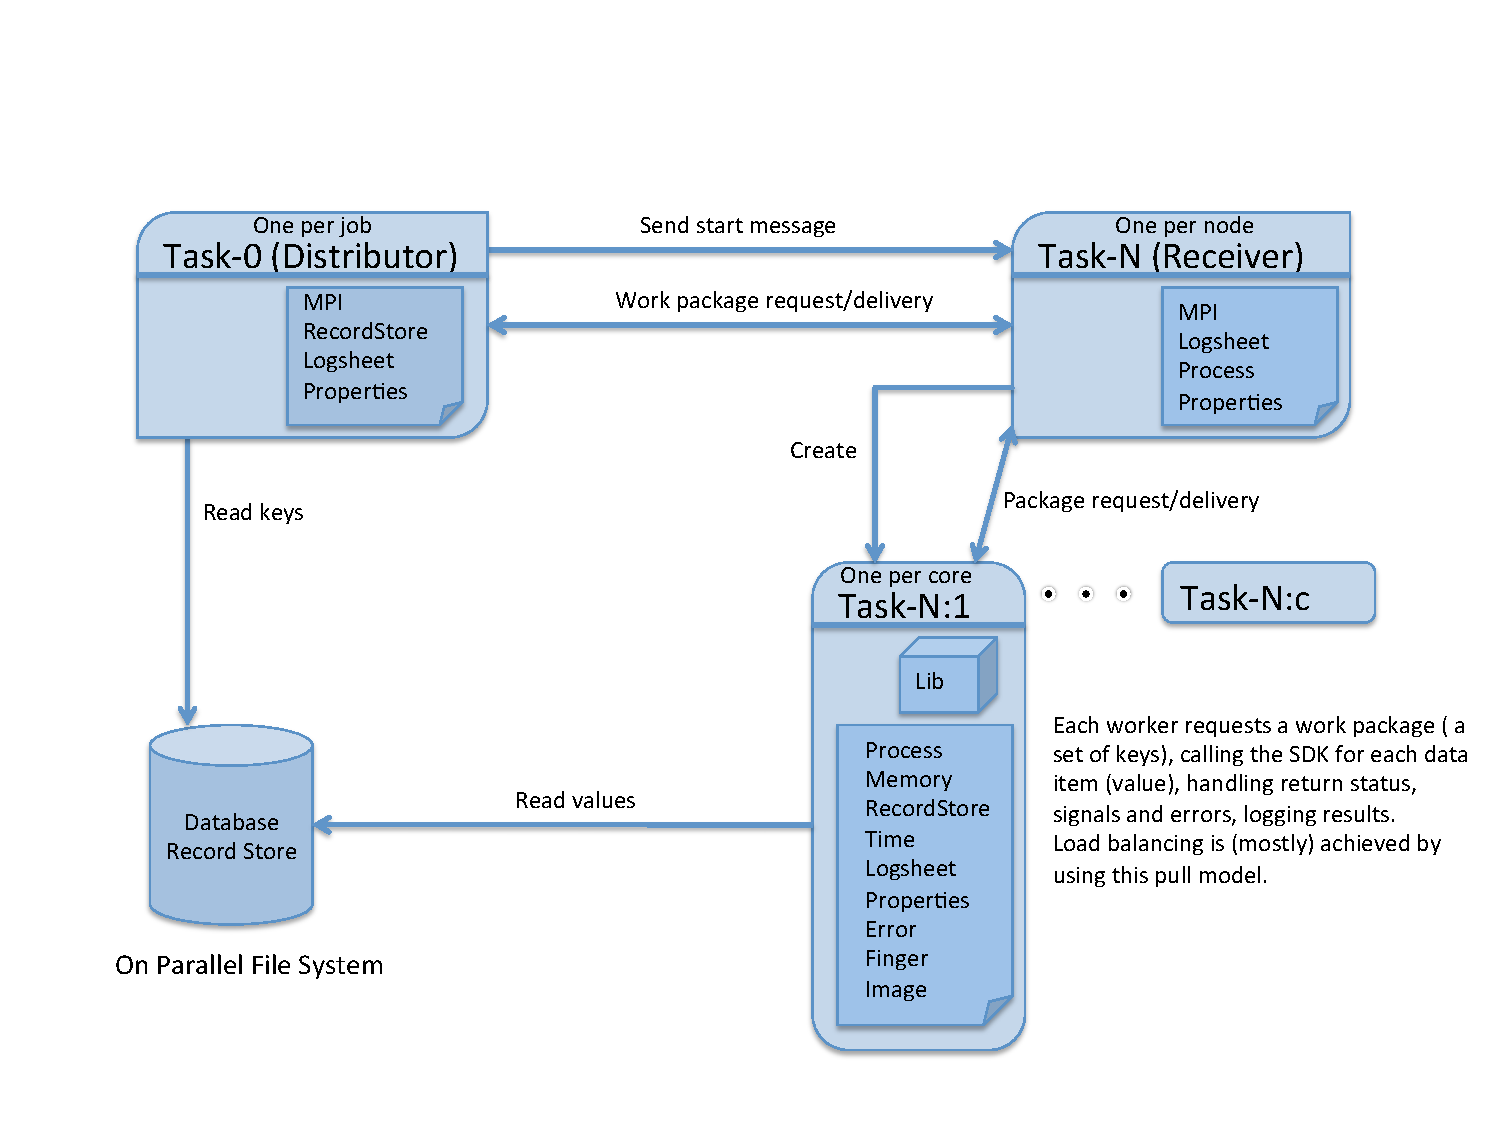
\includegraphics[width=\textwidth]{ParallelJob}
	\caption{MPI Parallel Job Processes and Data Flow}
	\label{fig:paralleljob}
\end{figure}

\section{Work Package}
\label{sec-workpackage}

A \class{WorkPackage} object wraps a simple container of data
with some access methods. There is no information in this class pertaining to
the nature or format of the data; it is simply treated as an array of unsigned
integer values. However, clients of the class can store a value, the ``number
of elements'', that is transmitted along with the package. This value only
has meaning to the client, and is usually equivalent to the number of
larger-sized components making up the package. For example, this value may
be the number of records contained in the package. It is up to the client
(either an application or subclass) of \class{WorkPackage} to understand
how to separate the array into components.

\section{Distributor}
\label{sec-workpackagedistributor}

The \class{Distributor} is an abstract class than encapsulates the MPI
functionality and is responsible for distributing work packages to other
elements within the MPI job (the receivers). However, this class
is also responsible for coordinating the startup and shutdown of the receiver
tasks. MPI messages are used for this coordination. An MPI job may fail to
start if the distributor fails to initialize, or if none of the receivers
initialize.

One method of the \class{Distributor} class, \code{createWorkPackage()},
is implemented by child classes. This method creates a single work package
with the knowledge of how the elements of the package are to be stored
in the package's data buffer. \class{RecordStoreDistributor} is an
implementation of \class{Distributor}.

\subsection{Record Store Distributor}
\label{sec-recordstoredistributor}

\class{RecordStoreDistributor} reads records from a \class{RecordStore},
packs record keys, and optionally, values into a \class{WorkPackage}. This
class inherits all of the MPI communication, intra-job coordination, logging,
and other aspects of the \class{Distributor} parent class.

An application can create an instance of a \class{RecordStoreDistributor}
with the name of a record store in order to distribute records for
processing across the MPI job. \lstref{lst:mpiappmain} shows an
example section of code to create a record store distributor. In this
type of application there is no need for the application code to refine
any of the Framework classes.

\section{Receiver}
\label{sec-workpackagereceiver}

The \class{Receiver} class encapsulates all the MPI messaging needed to
participate in the MPI job as the receiver of data to be processed. In
addition, this class is responsible for starting other processes that
perform work on the actual data from the work package.

It is expected, as part of the MPI job, that a single receiver process
will be started on each node in the job. More than one can be started,
however. Each receiver starts one or more child processes to
consume data. The receiver monitors each worker process and
will instruct them to shut down when the job is finished (no more data),
early termination signals are received, or in the case of errors
encountered by the receiver.

By keeping the data consumers as separate processes, the receiving half
of the MPI job can be more robust as a premature termination of a worker
process (due to memory corruption, for example) will not affect other
workers.

\section{Work Package Processor}
\label{sec-workpackageprocessor}

The \class{WorkPackageProcessor} class is pure-virtual and provides the
interface for any class that uses a \class{WorkPackage} to receive data from
the MPI Framework.
\class{WorkPackageProcessor} also maintains a \class{Logsheet} object which
can be used by subclasses to store log messages.

Implementations of this class can be considered to have dual responsibilities.
First is the management of common state used by all workers (Task-N:c in
\figref{fig:paralleljob}); creating state data shared by all workers, for
example.
Second, as a factory to create a package consumer for the worker process.

The \code{performInitialization()} method is called before the \class{Receiver}
object forks and creates the worker processes. The application can use this
function to load a large data set into memory (taking advantage of copy-on-write
memory semantics present in most modern operating systems), or perform any
node-local setup that should only be done once the MPI job has begun.

\code{newProcessor()} returns a new instance of the package processor.
This method is called by the Framework when a new process is started by the
receiver to consume work packages sent by the distributor. This method is a
factory, creating new instances of the \class{WorkPackageProcessor}
implementation. Therefore, it must create a ``fully-formed'' object that may
have different state than that created by the class constructor. An example
would be creating an output log file with record information.
This output file would not be created in the constructor because the
object returned from that will not process a work package; it is the factory
object.

It is the
responsibility of the \code{newProcessor()} method to ensure there is no
resource contention between instances of this class, as the methods of this
object will be executed within a separate process. The
\code{MPI::generateUniqueID()} function can be used to create a name string
that to identify the process.

\subsection{Record Processor}
\label{sec-recordprocessor}
\class{RecordProcessor} is a partial implementation of 
\class{WorkPackageProcessor} and defines the \code{processWorkPackage()}
of the \class{WorkPackageProcessor} interface; other methods are declared as
pure-virtual and must be implemented by a child class. In addition,
\class{RecordProcessor} declares a new pure-virtual method,
\code{processRecord()} to be implemented by a subclass to process a single
record from the record store. In summary, \class{RecordProcessor} removes
records from the work package to be processed within the subclass,
which is defined by the application.
See~\lstref{lst:mpiappclasses} and \lstref{lst:mpiappimpl} for a example of
such an implementation.

\section{MPI Resources}
\label{sec-mpiresources}
Every MPI job depends on a set of properties contained within a text file.
These properties are read into a \class{Properties} object contained within
the \class{Resources} object.

The core MPI classes (\class{Distributor} and \class{Receiver}) use these
properties:
\begin{description}
\item[Workers Per Node] Used by the receiver process to start the
required number of workers;
\item[Logsheet URL] Use by distributor and receiver processes
(and children) to open the log.
\end{description}

The \verb=Logsheet URL= property is optional, and if present all MPI Framework
trace messages will be written to the specified logging target. Two types of
\URL schemes are allowed: \verb=file://= and \verb=syslog://=, corresponding
to the types of \class{Logsheet} classes (\secref{sec-logging}) in the
Framework.

Subclasses and other components of the MPI Framework may add properties as
needed, usually to the same file as the above properties. Record-based jobs
(using \class{RecordStoreDistributor} and \class{RecordProcessor}), for example,
have these additional properties:

\begin{description}
\item[Input Record Store] The input record store;
\item[Chunk Size] How many record keys or key-value pairs to place into a
work package.
\end{description}

For a record store job, an example properties file might be:
\begin{verbatim}
Input Record Store = test.rs
Chunk Size = 7
Workers Per Node = 3
Logsheet URL = file://mpi.log
\end{verbatim}

Applications can add one or more properties to the file as needed. One example
would be a URL for a Logsheet used only by the application.

\section{MPI Runtime}
\label{sec-mpiruntime}

The \class{Runtime} class is the interface between the application and the
MPI runtime environment. The \code{argv} and \code{argc} parameters
to the \code{main()} function as passed through to the \class{Runtime}
object, then onto the core OpenMPI functions. The \class{Runtime} object 
also sets up a signal handler for the job, and starts the \class{Distributor}
and \class{Receiver} processes.  A method is also provided for the application
to abort the MPI job, providing for a somewhat clean shutdown.

On of the key features of an MPI job under the Framework is premature shutdown
with minimal loss of work. Three types of exit condition can be set by sending
a signal to the distributor, receiver or worker processes. 

\begin{description}
\item[SIGQUIT] Exit when the current work package is exhausted;
\item[SIGINT] Exit when the current work item is finished (``quick exit'');
\item[SIGTERM] Exit immediately (``term exit'').
\end{description}

For the normal exit and quick exit cases, a clean shutdown is performed for
the distributor, receivers, and all worker processes. For term exit, each
worker process is terminated immediately and therefore cannot finish processing
the current work item. However, distributors and receivers will shutdown in a
clean manner.

Any of the signals can be sent to the distributor process, which then sends
messages to the receivers. In addition, if a signal is sent to a receiver, or
worker process, only that process (receiver or worker) is affected, but the
termination condition is communicated ``up'' the chain. By selectively sending
signals to certain processes, a user can shutdown the entire job (send to the
distributor), an entire node (send to the receiver on that node), or a single
worker. A worker receiving a signal sends a message back to the receiver.
Likewise, a receiver will communicate the shutdown state back to the
distributor.

\section{Logging}
\label{sec-mpilogging}
In order to aid tracing and debugging of a parallel job, the MPI Framework
can be configured to write trace messages to the log storage. These trace
messages are logged as debug messages instead of normal entries.
The type and location of the log is given to the 
Framework by using a URL as a property when starting the MPI
job (see~\secref{sec-mpiresources}).

When the URL for a log is the {\tt file://} type, the MPI Framework will create
several log files on the node where it runs. The reason for this is that during
\class{Receiver} processing, one or more worker processes are created in
addition to the main receiver process. Each of these processes requires
exclusive access to the file-based log sheet in order to avoid conflicts with
the log entry commitment.
The log files will be named with the property value
as a prefix, and the hostname/MPI task number/process ID added as a suffix.
For example, if the property is \verb=file://mpijob.log=, a log file might
have a name of \verb=mpijob.log-node01-1-12345=.

To aid logging within the application, access to the \class{Logsheet} opened
by the Framework is available via the class whose interface is implemented
within the application, \class{WorkPackageProcessor}, for example.

Two wrapper functions, \code{MPI::logMessage()} and \code{MPI::logEntry()},
are provided in order to ``safely'' log. These functions handle all errors
from the \class{Logsheet} object, and will turn off log message commitment
once an error occurs. The Framework and application can continue processing.

\section{MPI Framework Applications}
\label{sec-mpiapp}

An application of the MPI Framework is responsible for implementing several
functions declared in the Framework, requiring subclassing of the MPI classes.
In this section an example application that processes records from a store will
be described. 

\lstref{lst:mpiappclasses} shows the header file that declares a subclass of
\class{RecordProcessor}. The \code{newProcessor()},
\code{performInitialization()}, and \code{processRecord()} methods are those
required to complete an implementation of \class{RecordProcessor}.

\begin{lstlisting}[caption={MPI Framework Application Classes}, label=lst:mpiappclasses]
class TestRecordProcessor : public BiometricEvaluation::MPI::RecordProcessor {
public:
        TestRecordProcessor(
            const std::string &propertiesFileName);
        ~TestRecordProcessor();

        std::shared_ptr<BE::MPI::WorkPackageProcessor>
        newProcessor(std::shared_ptr<BE::IO::Logsheet> &logsheet);

        void
        performInitialization(std::shared_ptr<BE::IO::Logsheet> &logsheet);

        void processRecord(const std::string &key);

        void processRecord(
            const std::string &key,
            const BE::Memory::uint8Array &value);

protected:
private:
        std::shared_ptr<BE::IO::Logsheet> _recordLogsheet;
};

\end{lstlisting}

Next, \lstref{lst:mpiappimpl} shows the implementation of the class methods. In
this simple example, each record is acknowledged with a log entry.

Also shown in several of the methods is the use of the \class{Logsheet} object
provided to the application by the Framework, along with wrapper functions,
\code{logMessage()} and \code{logEntry()}.

The application also creates its own
\class{Logsheet} object in order to separate Framework log messages from the
application messages when processing the actual record. In error cases, the
Framework log is used in order to keep the set of calls from the Framework
to the application in sequence and package processing together.

\begin{lstlisting}[caption={MPI Framework Application Implementation}, label=lst:mpiappimpl]
#include <be_mpi_receiver.h>
#include <be_mpi_recordstoredistributor.h>
#include <be_mpi_runtime.h>

#include "test_be_mpi.h"

using namespace BiometricEvaluation;

static const std::string DefaultPropertiesFileName("test_be_mpi.props");

/*
 * Implementations of the MPI RecordProcessor class interface.
 * Calls the parent constructor to manage the properties file name.
 */
TestRecordProcessor::TestRecordProcessor(
    const std::string &propertiesFileName) :
    RecordProcessor(propertiesFileName)
{
}

TestRecordProcessor::~TestRecordProcessor()
{
}

/*
 * Factory object: Create a new instance of the TestRecordProcess
 * that will work on work package records. Each instance gets
 * its own instance of the log sheet.
 */
std::shared_ptr<BiometricEvaluation::MPI::WorkPackageProcessor>
TestRecordProcessor::newProcessor(
    std::shared_ptr<IO::Logsheet> &logsheet)
{
        std::string propertiesFileName =
            this->getResources()->getPropertiesFileName();
        TestRecordProcessor *processor =
            new TestRecordProcessor(propertiesFileName);
        processor->setLogsheet(logsheet);

        /*
         * If we have our own Logsheet property, and we can open
         * that Logsheet, use it for record logging; otherwise,
         * create a Null Logsheet for these events. We use the
         * framework's Logsheet for tracing of processing, not
         * record handling logs.
         */
        std::string url;
        std::unique_ptr<BE::IO::PropertiesFile> props;
        try {   
                /* It is crucial that the Properties file be
                 * opened read-only, else it will be rewritten
                 * when the unique ptr is destroyed, causing
                 * a race condition with other processes that
                 * are reading the file.
                 */
                props.reset(new BE::IO::PropertiesFile(
                    propertiesFileName, IO::READONLY));
                url = props->getProperty(
                    TestRecordProcessor::RECORDLOGSHEETURLPROPERTY);
        } catch (BE::Error::Exception &e) {
                url = "";
        }
        processor->_recordLogsheet = BE::MPI::openLogsheet(
            url, "Test Record Processing");

        std::shared_ptr<BiometricEvaluation::MPI::WorkPackageProcessor> sptr;
        sptr.reset(processor);
        return (sptr);
}

/*
 * Factory object: Simply log our call.
 */
void
TestRecordProcessor::performInitialization(
    std::shared_ptr<IO::Logsheet> &logsheet)
{
        this->setLogsheet(logsheet);
        MPI::logMessage(
            *logsheet.get(), std::string(__FUNCTION__) + " called");
}

/*
 * Helper function to log some information about a record.
 */
static void
dumpRecord(
    BE::IO::Logsheet &log,
    const std::string key,
    const Memory::uint8Array &val)
{
	log << "Key [" << key << "]: ";
	/* Dump some bytes from the record */
        for (uint64_t i = 0; i < 8; i++) {
                log << std::hex << (int)val[i] << " ";
        }
        log << " |";
        for (uint64_t i = 0; i < 8; i++) {
                log << (char)val[i];
        }
        log << "|";
        BE::MPI::logEntry(log);
}

/*
 * The worker object: Log to the Framework Logsheet, obtain the data for
 * the record, and log some information to the record Logsheet.
 */
void
TestRecordProcessor::processRecord(const std::string &key)
{
        BE::IO::Logsheet *log = this->getLogsheet().get();
        BE::MPI::logMessage(*log, "processRecord(key) called.");
        Memory::uint8Array value(0);
        std::shared_ptr<IO::RecordStore> inputRS =
            this->getResources()->getRecordStore();

        try {
                inputRS->read(key, value);
        } catch (Error::Exception &e) {
                *log << "Could not read record: " + e.whatString());
        }
	BE::IO::Logsheet *rlog = this->_recordLogsheet.get();
       	dumpRecord(*rlog, key, value);
}

/*
 * The worker object: Log to the Framework Logsheet, and log some record
 * information to the record Logsheet.
 */
void
TestRecordProcessor::processRecord(
    const std::string &key,
    const BiometricEvaluation::Memory::uint8Array &value)
{
        BE::IO::Logsheet *log = this->getLogsheet().get();
        BE::MPI::logMessage(*log,"processRecord(key, value) called");

        BE::IO::Logsheet *rlog = this->_recordLogsheet.get();
        dumpRecord(*rlog, key, value);
}

\end{lstlisting}

\begin{lstlisting}[caption={MPI Framework Application Main}, label=lst:mpiappmain]
int
main(int argc, char* argv[])
{
        /*
         * It is important that the MPI runtime environment be started
         * prior to any other activity that may result in premature
         * termination. Therefore, participate in the MPI environment, but
         * don't create a Receiver or Distributor until any local items
         * are take care of.
         */
        MPI::Runtime runtime(argc, argv);

        std::unique_ptr<MPI::RecordStoreDistributor> distributor;
        std::unique_ptr<MPI::Receiver> receiver;
        std::shared_ptr<TestRecordProcessor> processor;

        /*
         * If there is any argument to the program, use keys only as the
         * record distribution method. Otherwise, use keys and values.
         */
        bool includeValues;
        if (argc == 1) {
                MPI::printStatus("Test Distributor and Receiver, keys only");
                includeValues = false;
        } else {
                MPI::printStatus("Test Distributor and Receiver, keys and values");
                includeValues = true;
        }
        try {
                distributor.reset(
                    new MPI::RecordStoreDistributor(propFile, includeValues));

                processor.reset(new TestRecordProcessor(propFile));

                receiver.reset(new MPI::Receiver(propFile, processor));

                runtime.start(*distributor, *receiver);
                runtime.shutdown();
        } catch (Error::Exception &e) {
                MPI::printStatus("Caught: " + e.whatString());
                runtime.abort(EXIT_FAILURE);
        } catch (...) {
                MPI::printStatus("Caught some other exception");
                runtime.abort(EXIT_FAILURE);
        }

        return (EXIT_SUCCESS);
}

\end{lstlisting}

%--------------------------------------------------------------------------
% Generate and add the bibliography to the table of contents
%--------------------------------------------------------------------------
\renewcommand\bibname{References}
\bibliographystyle{plain}
\bibliography{BECommonFramework}
\addcontentsline{toc}{chapter}{References}
